\chapter{Electromagnetic Worldlines - Numerical Methods and Results}
\label{ch:numerical}

The ultimate goal of this project is to build a general numerical method. In order to test results 
it is necessary to test smaller cases carefully first.  Despite the emphasis on planar geometries,
we have tried to develop methods that would be well suited to more complicated geometries,
and test them in the simple geometry.  In this case we can carefully test their convergence properties
as the path resolution is increased.  

Even in a planar geometry we have had to develop an array of tools to make the worldline methods tractable.
The TM polarization is by far the hardest to deal with, and has prompted most of these developments.
The same developments can be used to enhance the TE polarization, as well as existing Dirichlet
worldline methods.

We will discuss techniques path construction, Monte Carlo sampling of the path starting points $x_0$
and path-time $\cT$.  In the case of the TE polarization, these are all quite straightforward.  
The TM polarization displays large numerical fluctuations, which must be tempered by changing the methods
used to construct the paths.  The essence of these methods is importance sampling, beyond what is manifestly
obvious from the form of the path integral.    

The numerical results will be compared against the expected efficiencies $\eta(\chi)$ and $\gamma(\chi)$.
The worldline method tends to straightforwardly reproduce the expected distance dependence due to the
integration over $\cT$, as was briefly discussed in Sec.~\ref{sec:worldline_distance_dep}. 
That is still true within the for electromagnetic worldlines. 
All of the simulations are carried out for a fixed $\chi$ in the far-field limit, but we will discuss how
to generalize the simulations to allow dispersion.  
The computations at fixed $\chi$ are useful indicators for how the full dispersion simulations.
In the Casimir effect, each frequency contributes independently, so for a particular frequency $\chi(i\omega)$
is effectively constant.  Since $\chi(i\omega)$ is a positive real constant, that diverges in some cases
(such as metals), it is necessary to see how the worldline algorithm performs across a whole range of susceptibilities.

The numerical results on the TE Casimir energies were published in Ref.~\cite{Mackrory2016}.

\section{TE Casimir Numerics}

In this section we will discuss numerically simulating the TE Casimir and Casimir--Polder energies 
from the worldline expressions in Eqs.~(\ref{eq:TE_Casimir}) and (\ref{eq:TE_Casimir_Polder}).
We will first discuss path generation, sampling starting positions $\vect{x}_0$ and path-times $\cT$,
and evaluating the dielectric path-average $\langle \epsr\rangle$.  % Despite working with expressions adapted to planar
% media, we will endeavour to develop general purpose numerical methods that would work in more general
% geometries.  

\subsection{Path generation}

The principal element of the worldline method is evaluating a potential along an ensemble of Gaussian
paths.  This allows the $N$-dimensional integral over positions to be efficiently evaluated in a 
Monte Carlo fashion via $N_p$ sample paths.
It is of primary importance to be able to efficiently generate these Gaussian sample paths. 

\subsubsection{Open Brownian Bridges: V-loop construction}

The v-loop algorithm is derived by decoupling the product of $N$ Gaussian probability densities 
into $N-1$ independent Gaussian deviates~\cite{Gies2003}.
Since we will need to construct open and closed Brownian bridges of fixed length $N$, we will derive the v-loop algorithm
for open paths, as closed paths are a special case of open paths.  

Consider a Gaussian density of $N$ steps in one dimension, where the end points $x_0$ and $x_N$ 
are fixed:
\begin{equation}
  P(x_1,\ldots,x_{N-1}) = (2\pi\Delta\cT)^{-N/2}\exp\left[-\sum_{j=0}^{N-1}\frac{(x_{j+1}-x_j)^2}{2\Delta\cT}\right].
  \label{eq:Gaussian_distrib}
\end{equation}
It is convenient to define a shifted, normalized variable $y_k = (x_k-x_0)/\sqrt{\Delta \cT}$.
The exponent for the product of coupled Gaussians is
\begin{equation}
X = \frac{y_1^2}{2}+\frac{(y_2-y_1)^2}{2}+\cdots+\frac{(y_{N-1}-y_{N-2})^2}{2}+\frac{(\Delta x-y_{N-1})^2}{2},
\label{eq:Xexp}
\end{equation}
where $\Delta x :=(x_N-x_0)/\sqrt{\Delta \cT}$.  
The exponent~(\ref{eq:Xexp}) can be decoupled by completing the square repeatedly.
The process starts at one end of the path $y_{N-1}$.  It is convenient to
introduce a variance $\sigma^2_{N-1}=1$ as a bookkeeping device.
It is possible to quickly develop recursion relations for how the resulting means and variance scale.  
\begin{align}
  & \frac{(y_{N-1}-\Delta x)^2}{2\sigma_{N-1}^2}+\frac{(y_{N-1}-y_{N-2})^2}{2} \nonumber \\
  &= \frac{\sigma^2_{N-1}+1}{2\sigma_{N-1}^2}
  \left(y_{N-1} - \frac{\sigma_{N-1}^2y_{N-2}+\Delta x}{\sigma_{N-1}^2+1}\right)^2 + \frac{(y_{N-2}-\Delta x)^2}{2(\sigma^2_{N-1}+1)}
  % &= \frac{1}{2c_{N-1}}
  % \left(y_{N-1} - c_{N-1}y_{N-2}-\frac{\Delta x}{\sigma_{N-1}^2+1}\right)^2 + \frac{(y_{N-2}-\Delta x)^2}{2(\sigma^2_{N-1}+1)}\\
\end{align}
where $\sigma_{N-2}:=\sigma_{N-1}+1$, and $c_{N-1} = \sigma_{N-1}^2/(\sigma_{N-1}^2+1)$.
After each completion of the square $\sigma_{N-j}\rightarrow \sigma_{N-j+1}+1$.  After repeating the process $N-1$ times
the exponent is 
\begin{equation}
  X = \frac{\Delta x^2}{2N} + \sum_{j=1}^{N-1} \frac{z_j^2}{2},
\end{equation}
where 
\begin{equation}
  z_j = \frac{1}{2c_j}\left(y_j - c_jy_{j-1}-\frac{\Delta x}{N-j+1}\right)^2,\label{eq:zj}
\end{equation}
and 
\begin{equation}
  c_j = \frac{N-j}{N-j+1}.
\end{equation}
The $z_j$ are decoupled standard normal variables.  Once the $z_j$ have been sampled the 
transformation (\ref{eq:zj}) can be inverted to find the path,
\begin{equation}
  x_k = x_0 + \frac{x_N-x_0}{N-k+1}+c_kx_{k-1} + \sqrt{c_k\Delta\cT}z_k.\label{eq:open_vloop}
\end{equation}
\comment{double check counting?}
There is then an remaining normalization factor of $e^{-(x_N-x_0)^2/(2\cT)}/\sqrt{2\pi\cT}$,  
which accounts for the Jacobian $\prod_{j}c_j=N^{-1}$ from changing variable.
This normalization is also the normalization factor derived in Eq.~\ref{eq:Gaussian_normalization}.
An integral against the probability density~(\ref{eq:Gaussian_distrib}) could be evaluated as follows,
\begin{equation}
  I = \int \prod_{j=1}^{N-1}dx_j P(x_1,\ldots,x_{N-1})f(x_1,\ldots,x_N)
  = \frac{e^{-\frac{(x_1-x_N)^2}{2\cT}}}{\sqrt{2\pi \cT}}\dlangle f\drangle_{x(t)},
\end{equation}
where the ensemble average is taken over open Brownian bridges betwen $x_0$ and $x_N$.
The limit of closed paths can be easily taken by setting $x_N-x_0=0$.
The v-loop construction is also straightforwardlygeneralized to vector Brownian bridges.  
This procedure allows the generation of a unit loop for $\cT=1$, which can then be integrated over
multiple starting points $x_0$ and total path-times $\cT$.  A closed unit Brownian bridge can be constructed 
as
\begin{equation}
  B_k = c_kB_{k-1} + \sqrt{\frac{c_k}{N}}z_k.\label{eq:unit_vloop}
\end{equation}
A shifted, scaled Brownian bridge can then be constructed as
\begin{equation}
  x_k = x_0 + \sqrt{\cT} B_k.
\end{equation}

The original v-loop algorithm used centered paths, where the average position $\langle x\rangle$ is subtracted from the path~\cite{Gies2003}.
This requires first constructing the Brownian bridge, and then subtracting off the mean position.  
This is inconvenient if the path is being generated on the fly 
without storage, or if there are stochastic elements to path construction.    
In Casimir--Polder applications (or when computing the stress-energy tensor~\cite{Schafer2016}),
 it is better to consider paths emanating from a single point $\vect{x}_0$.
  The starting point corresponds to the atom's location, or the point where
the stress-energy tensor is being computed.  

\subsection{Monte-Carlo sampling}

To evaluate the Casimir energy it is necessary to integrate the results for a single path over all
starting points $\vect{x}_0$, path-times $\cT$, and average over an ensemble of paths.
% The rationale for also sampling over times is to allow further ensemble averaging over paths,
% and times. 
The original Gies\etal computations emphasized computing the total $\cT$ integral for each path~\cite{Gies2003}.
For Dirichlet worldlines, the path integrand is either zero or one based on whether the path intersects
all of the bodies.  This makes evaluating the integral a tractable problem, since 
it only requires finding the set of times $\{\cT_k\}$ when paths enter the body, and evaluating 
$\int_{\cT_0}^{\cT_1} d\cT\,\cT^{-(1+D/2)}$ during those  times the integral is nonzero.
For example, in their paper computing forces in a sphere-plane geometry Weber and Gies find analytical
expressions in terms of $\vect{x}_0$ and $\cT$ for when each random path will intersect both bodies~\cite{Weber2010}.
The remaining integrals over $\vect{x}_0$ and $\cT$ can be evaluated on a path-wise basis.

However, for the dielectric integrands that the TE and TM path integrals require, 
the integrand changes value based on how many points are inside the surface.  For a path of length $N$, this direct method would
require finding all $N$ intersection times and then evaluating the integrals.  
This becomes impractical for large $N$, as a large computational effort  must be expended on even a single path.  
This becomes even more burdensome once the integral over the starting position is accounted for.

Since the $N$-fold integral over positions is being handled in a Monte Carlo fashion, it makes sense to 
treat the remaining integrals over the starting position $\vect{x}_0$ and path-times $\cT$ in the same manner.
Each path can be evaluated for a single pair of $\vect{x}_0$ and $\cT$, where those are picked from suitable
distributions, governed by the form of the integral.  This is a form of importance sampling, which 
is a powerful tool for accelerating Monte Carlo numerical computations~\cite{Asmussen2007, Glasserman2004}.
This style of importance sampling goes beyond just using the Gaussian probability density to evaluate the 
spatial integrals over the intermediate positions $\vect{x}_k$.  In this case, the importance sampling
relies on knoweldge on which positions and times the most to the integral. 
This Monte Carlo sampling of $x_0$ and $\cT$ also extends the number of independent paths that can be averaged over, which 
is essential for good convergence.   

\subsubsection{Sampling Path-Times from a Power Law}

The simplest method of sampling path-times, is to exploit the presence of $\cT^{-(1+D/2)}$ in the integral.
For a particular path, the renormalized TE integrand is only non-zero after the path touches all of the bodies,
which occurs at some path-time $\cT_0$.\footnote{For a Brownian motion $\vect{x}(t)$,
the term ``first-touching time'' is reserved for the first time $t_0$ along a path that a Brownian bridge intersects a surface: $\vect{x}(t_0)=d$. 
This is distinct from the first path-time $\cT$ when any section of the scaled path intersects a surface.
}
For $\cT>T_0$,  the extent of the path grows as $\sqrt{\cT}$, so the integrand $(\langle\epsr\rangle^{-\alpha}-1)$ 
increases as more points enter the bodies.  
However, the $\cT^{-(1+D/2)}$ factor decreases the contributions from large path-times $\cT$.
These facts suggest sampling $\cT$ from a probability distribution 
\begin{equation}
  P(\cT;\cT_0,m)= \frac{(m-1) \cT_0^{m-1}}{\cT^m}\Theta(\cT-\cT_0),\label{eq:Tpower_law}
\end{equation}
where $m>1$ and $\cT_0>0$.  This requires being able to estimate the value of the first-contact time $\cT_0$.  
For the example of paths starting between parallel planes $\cT_0=\text{min}[\left(\frac{-d_1-x_0}{B_-}\right)^2,
\left(\frac{d_2-x_0}{B_+}\right)^2]$ where $d_1<x_0<d_2$, and $B_\pm$ are the maximum and minimum points
of the unit Brownian path.  The path-time $\cT_0$ is the lowest bound on when the path will touch the relevant bodies.
In computing Casimir interaction energies, the path must touch \emph{all} of the bodies, while in Casimir--Polder
calculations, the path must touch \emph{any} of the bodies to contribute.  

Samples from the distribution~(\ref{eq:Tpower_law}) can be generated by inverting the cumulative probability distribution.
(This sort of inversion is a general purpose method of generating random deviates from a distribution~\cite{NumRecipe,Devroye2003}.)
In this case, the inversion requires a solution $\cT$ to
\begin{equation}
  r=(m-1) \cT_0^{m-1}\int_{\cT_0}^\cT dt\, t^{-m}
\end{equation}
where $r\in [0,1]$ is a uniform random number and $\cT$ is the desired deviate.    
This can be easily solved, with the result that
\begin{align}
%  r&=(m-1) \cT_0^{m-1}\frac{1}{m-1}\left(\frac{1}{\cT_0^{m-1}}-\frac{1}{\cT^{m-1}}\right)\\
%  \left(\frac{\cT_0}{\cT}\right)^{m-1}&= (1-r)\\
 \cT= \frac{\cT_0}{(1-r)^{1/(m-1)}}.
\end{align}
The lower-bound $\cT_0$ can be easily found in simple geometries on a path-wise basis. Deviates
$\cT$ can then be generated for each path, where each path is then guaranteed to contribute.  

In a more complicated arrangement of bodies, the lower-bound $\cT_0$ could be found via root-finding,
to find the minimum path-time that the path touches all of the relevant bodies.  It is important for 
$\cT_0$ to be a lower bound on the first time the integrand is nonzero, otherwise this method will miss 
part of the integral.  However, $\cT_0$ should not be set too low, as otherwise numerous samples will
be made which generates paths that are too small to contribute.  

\subsubsection{Sampling Starting Positions}

The integral over the starting point $x_0$ can also be evaluated in Monte-Carlo fashion by exploiting some knowledge 
about the form of the integrand.  
For points $x$ far from all bodies located around the origin, the expected minimum path-time when the integrand is nonzero 
is $\cT_0\sim x^2$.
If the extent of the finite bodies is $d_{\text{max}}$, then there is also a maximum time $\cT_1$ for when the path is so large 
that it does not intersect the bodies anymore (this may be infinite in some geometries).
In that case, and approximating the integrand $(\langle\epsr\rangle^{-1}-1$ by its strong-coupling limit,
the path-time integral is approximately 
\begin{equation}
  \int_{\cT_0}^{\cT_1} \frac{d\cT }{\cT^{1+D/2}} = \frac{1}{x^{D}}-\frac{1}{d_{\text{max}}^D}.
\end{equation}
This suggests that the contribution from points far from the bodies scales at most as $x^{-D}$.  
In between the bodies, the contribution from each starting position is roughly uniform, since each path must have sufficient extent
to touch all bodies.  
This occurs for times $\cT\sim d_0^2$, where $d_0$ is the separation between bodies.    
In a one-dimensional geometry, embedded in a four-dimensional space-time, 
these considerations suggest sampling from 
\begin{equation}
  P_x(x;d_0):= \frac{3}{8d_0}\left\{ \begin{array}{cc}
    1  & |x|<d_0\\
    \dfrac{d^4_0}{|x|^4} & |x|>d_0
  \end{array}
\right.\label{eq:xPower_law}.
\end{equation}
This reasoning can be easily extended to higher dimensional problems,
where a sphere of radius $d_0$ should bound all of the interfaces between the bodies.
Outside of that sphere, the sampling would again fall off as $|x|^D$.  
While it may be possible to develop sampling procedures better suited to a particular geometry, 
this provides a general purpose way of sampling the starting points for Casimir worldline path integrals.

\subsubsection{Evaluating the Dielectric Path Average}

Once a path is constructed, the rest of the path integral integrand can be sampled along that path.
For example, the path average of the dielectric can be evaluated as 
\begin{equation}
  \langle\epsr\rangle = \frac{1}{N}\sum_{k=1}^N\epsr(x_k).
\end{equation}
This corresponds to the trapezoidal rule for evaluating the path-average, 
\begin{equation}
  \langle\epsr\rangle = \frac{1}{\cT}\sum_{k=0}^{N-1}\int\limits_{k\Delta\cT}^{(k+1)\Delta\cT} dt'\, \epsr[x(t')]
  \approx = \frac{\Delta \cT}{N}\sum_{k=0}^{N-1}\frac{\epsr(x_k)+\epsr(x_{k+1})}{2}=\frac{1}{N}\sum_{k=1}^N\epsr(x_k)
\end{equation}
where the trapezoidal rule $\int_a^b dx\,f(x)=(b-a)[f(a)+f(b)]/2$, was used for each time integral.
As discussed in \S 5.C.3 of Ref.~\cite{Mackrory2016}, the trapezoidal rule outperforms some improved methods.  
For example, in cases where $x_k$ and $x_{k+1}$ straddle a surface at $d$, the integral could be 
weighted by the fraction of the path increment inside the surface, $(x_{k+1}-d)/(x_{k+1}-x_k)$.
This reduces the contribution from path increments where one point just enters the surface.  
Unfortunately, this does not fix an opposing error: what about paths that come close to the surface but just 
miss it?  There is some finite probability that a sub-path between $x_k$ and $x_{k+1}$ would have entered the body, and given a greater 
contribution.  Since the reduction of the contribution is not offset, this more advanced method actually
fares worse than the straightforward trapezoidal method. 

\subsection{TE Casimir  and Casimir--Polder Energies - Plane-Plane}

These methods can be applied to computing the TE Casimir and Casimir--Polder energies.  
As a first step, let us consider the Casimir--Energy for an atom interacting with a dielectric half-space 
in the zero temperature, far-field limit.  The atom is located at the origin, with a dielectric half-space 
a distance $d$ away with a constant susceptibility $\chi$.

Fig.~\ref{fig:eff_TE_atom_wall} shows the numerical results for evaluating the TE Casimir--Polder path integral~(\ref{eq:TE_Casimir_Polder})
at a range of $\chi$.  
The TE Casimir--Polder energy is calculated numerically by evaluating
\begin{align}
  V\supTE\subCP-V_0 %&= -\frac{\hbar c\alpha_0}{8\pi^2}\biggdlangle \int_0^\infty\frac{d\cT}{\cT^{3}}\big(\langle \epsr\rangle^{-3/2}-1)  \biggdrangle \nonumber\\
  &=\biggdlangle \frac{\hbar c\alpha_0}{8\pi^2} \frac{1}{2\cT_0^{2}}\left(\frac{1}{\langle\epsr(x_k)\rangle^{-1/2}}-1\right) 
    \biggdrangle_{\vect{x}_k,\cT},\label{eq:TE_CP_num}
\end{align}
where $\dlangle \cdots\drangle_{\vect{x}_k,\cT}$ denotes an ensemble average over discrete Brownian bridges,
and times $\cT$.  
One dimensional Brownian bridges are constructed using the v-loop algorithm~(\ref{eq:unit_vloop}).
The minimum path-time $\cT_0$ is determined on a path-wise basis, based on solving $\sqrt{\cT_0}\text{max}(B_k)=d$.
The path-time is sampled for each path from Eq.~(\ref{eq:Tpower_law}), with $m=1+D/2=3$.
The path is then scaled, $x_k = \sqrt{\cT}B_k$, and the trapezoidal method is used to evaluate $\langle\epsr\rangle$
around each path.  The sojourn time per path $\langle\Theta(x-d)\rangle$ can be estimated once per path,
and then multiple $\chi$ can be computed at once using $\langle \epsr\rangle = 1+\chi\langle\Theta(x-d)\rangle$.
The results are then accumulated over many paths and times.  
The numerically calculated efficiency $\eta(\chi)$ is found by dividing the numerical results by the perfect-conductor result,
which cancels out the leading constants and the $d^{-4}$ distance dependence.

% As the results show, the agreement with between the numerical results
% and the analytical expression is excellent.  A more careful discussion of the numerical error is 
% deferred to Sec.~\ref{sec:TE_convergence}.
\begin{figure}
  \centering
 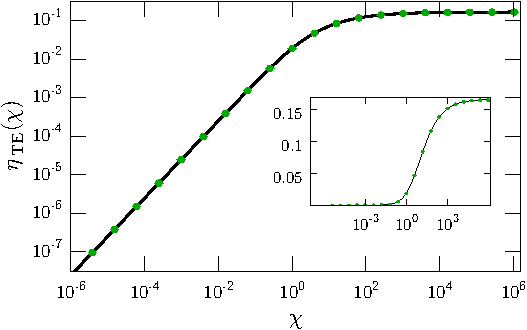
\includegraphics[width=0.8\textwidth]{fig/temp/eff_TE_atom_wall}
  \caption[Planar Casimir--Polder TE energy as function of $\chi$]
  {Planar Casimir--Polder TE energy as function of susceptibility $\chi$.  
    The simulations used $10^8$ paths, with $10^4$ points per path.
    Results for each $\chi$ were computed using the same ensemble of paths.
    The solid black line is the analytical result~(\ref{eq:etaTE}), and the points are the numerical
    values computed using Eq.~(\ref{eq:TE_CP_num}).
    (The inset is same data on a linear vertical scale.)
    }
  \label{fig:eff_TE_atom_wall}
\end{figure}

% Each path was generated with the v-loop algorithm~(\ref{eq:vloop}). 
% A single path-time $\cT$ was sampled for each path by sampling from Eq.~\ref{eq:Tpower_law}, 
% where $\cT_0$ is the smallest path-time that the part starting at $x_0$ would contact a planar surface a distance $d$ 
% away.  For TE integrands, a whole range of $\chi$ can be evaluated in parallel for a single path since 
% $\langle \epsr\rangle = 1+\chi\langle\Theta(x-d)\rangle$.  The path-averaged occupation time can be computed once for a 
% given path, and re-used to compute the Casimir--Polder energy for various $\chi$.  

% The numerically sampled values agree well with the analytical result for the 
% efficiency $\eta(\chi)$.  The efficiency is the ratio of the TE Casimir--Polder energy between an atom and a dielectric 
% to the total Casimir--Polder energy for an atom and a perfectly conducting plate.  This approaches $1/6$ in the 
% strong-coupling limit---the remainder of the Casimir--Polder energy is provided by the TM polarization, which
% will be discussed further in Sec.~\ref{sec:TM_numerics}.

\begin{figure}
  \centering
  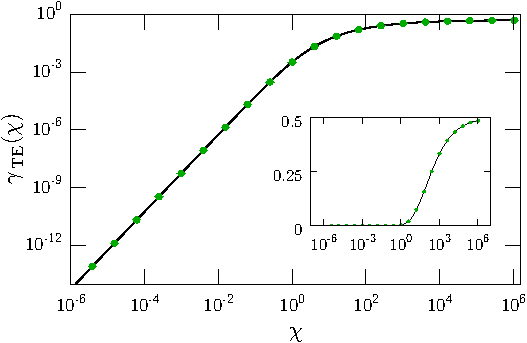
\includegraphics[width=0.8\textwidth]{fig/temp/eff_TE_2wall}
  \caption[Planar TE Casimir energy as function of $\chi$.]{
    Numerically calculated planar TE Casimir energy as function of $\chi$.
    The black lines show the analytical solution~(\ref{eq:gammaTE}), and the points show the numerical
    estimates.
    The simulations used $10^8$ paths, with $10^4$ points per path.  All values of $\chi$ were computed in parallel
    using the same ensemble of paths.
    (Inset is same data on a linear vertical scale.)}
  \label{fig:eff_TE_2wall}
\end{figure}

Fig.~\ref{fig:eff_TE_2wall} shows the numerically computed Casimir energy between two planar dielectric interfaces
a distance $d$ apart, with dielectric function $\epsr(x) = 1+\chi\Theta(-x+d/2)+\chi\Theta(x-d/2)$.  
This is computed numerically by evaluating
\begin{align}
  E\supTE\subCP-E_0 
  &=\biggdlangle \frac{\hbar c\alpha_0}{8\pi^2} \frac{1}{2\cT_0^{2}P_x(x_0)}
  \left(1+\frac{1}{\langle\epsrab(x_k)\rangle^{3/2}}-\frac{1}{\langle\epsra(x_k)\rangle^{3/2}}-\frac{1}{\langle\epsrb(x_k)\rangle^{3/2}}\right) \biggdrangle_{x_k,\cT,x_0},\label{eq:TE_Casimir_num}
\end{align}
The same procedure is similarto the one used for Casimir--Polder energies.  However, 
in this case there is an additional ensemble average over path starting position $\vect{x}_0$.
The starting positions are sampled from Eq.~(\ref{eq:xPower_law}), with $d_0=d$, 
which is twice the size of the region between the interfaces.  
In this case it is also necessary to keep track of $\langle \theta(x-d_2)\rangle$ and $\langle \theta(d_1-x)\rangle$.
The dielectric path average and the renormalized worldline integrand can also be quickly computed for multiple $\chi$.
One upshot of Monte Carlo sampling of positions is that this is \emph{much} faster than directly evaluating 
the position and path-time integrals on a path-wise basis.  In fact, evaluating the Casimir energy takes 
roughly the same time as the Casimir--Polder energy.  

\subsubsection{Scaling with N}
\label{sec:TE_convergence}
Some interesting scaling behaviour was found by examining the relative error between the numerical 
estimates and the exact analytical value.  
In this case the primary systematic error is due to the discretization of the path.
The path integral was derived under the assumption that $N\rightarrow\infty$, while the numerical
simulations use a discrete path with a finite $N$.  
There is an additional random error associated with the finite number of paths.   However, for $N_{\text{path}}$ paths,
this error scales as $N_{\text{path}}^{-1/2}$, as is typical for Monte Carlo sampling error.  This is what provides
the noise floor in Fig.~\ref{fig:conv_atom} and \ref{fig:conv_wall}.

\begin{figure}
  \centering
  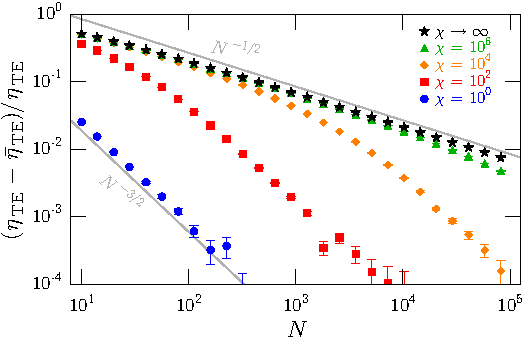
\includegraphics[width=0.8\textwidth]{fig/temp/conv_TEatomN3}
  \caption[Convergence of planar TE Casimir--Polder energy  as function of $N$.  ]{
    Convergence of planar TE Casimir--Polder energy as function of $N$.  
    Different values of $\chi$ use the same ensemble of paths.
    Simulations used $10^8$ paths, which sets the $10^{-4}$ noise floor.}
  \label{fig:conv_atom}
\end{figure}

\begin{figure}
  \centering
  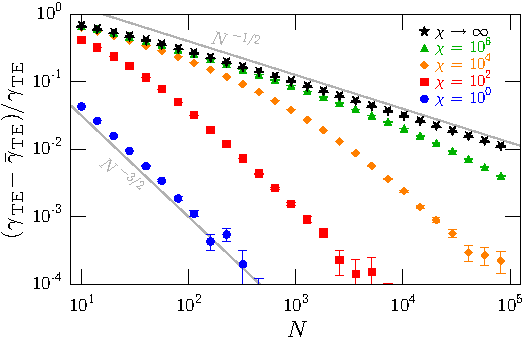
\includegraphics[width=0.8\textwidth]{fig/temp/conv_TE2wallN3}
  \caption[Convergence planar TE Casimir energy as function of $N$ for various $\chi$.]{
    Convergence planar TE Casimir energy as function of $N$ for various $\chi$, using the same ensemble of paths for all $\chi$.
    Simulations used $10^8$ paths, which sets the $10^{-4}$ noise floor.}
  \label{fig:conv_wall}
\end{figure}

As the path resolution $N$ varies for fixed $\chi$, the error shows two different scaling behaviours.  
In Ref.~\cite{Mackrory2016}, some arguments are given to explain this scaling, which will not be repeated here,
but we will explain the basic reasoning.  The numerical computations use discrete paths, 
while the path integral assumes $N$ is arbitrarily large.  Thus the paths considered by the path integral
have arbitrarily fine structure, with a non-zero probability to touch, or enter the dielectric body.
The discrete paths used in the numerical method miss those contributions.  

In the weak-coupling limit $\chi/N\ll 1$, the numerical estimate is dominated by accurately estimating the sojourn
time $\langle\theta\rangle$ for a given path.  Further increasing $N$ increases the accuracy of this 
estimate and renormalized integrand.  The $N^{-3/2}$ scaling can be estimated by integrating up the probability for a nonzero sojourn time
from each increment.  

In the strong-coupling limit $\chi/N\gg 1$, the integrand immediately saturates, and returns one.
Thus the dominant error comes from underestimating the time that this occurs.  The error scaling
is estimated by integrating up the probability that a continous path \emph{did} touch the surface
prior to the estimated first contact time.  This leads to a $N^{-1/2}$ scaling.

For a fixed $\chi$, the transition between both behaviours is observed at $N\sim\chi$. 
In the strict $\chi\rightarrow\infty$ Dirichlet limit, the numerical results and scaling 
arguments suggests that the numerical error will always scaled as $N^{-1/2}$.  However, for a finite
$\chi$ there is always such an $N$, although that $N$ grows linearly as the susceptibility increases.  

\section{TM Casimir Numerics}
\label{sec:TM_numerics}

Numerically calculating the Casimir energy due to the TM polarization is much harder than the TE case. 
This is due to the TM potential.
Even after regularization, and analytical path averaging, is still challenging to handle numerically.
We will develop a number of techniques to temper these difficulties that should have applications for more general Casimir worldlines.

The most daunting feature of the TM Casimir worldline is the singular TM potential.
 A closed form solution for the TM potential $V\subTM$ at a single planar boundary was found in Ch.~\ref{ch:feynman_kac}.
The ensemble averaged solution between points $x_k$ and $x_{k+1}$ in time $t$ is 
\begin{align}
  v_k(x_k,x_{k+1}):=\,&  \Bigdlangle e^{-\int_0^t dt'\, V\subTM(x-d)}\Bigdrangle_{x_k\rightarrow x_{k+1}} \\
   =\,& \Theta[X_{k,k+1}]\big[1 + \sgn(d-x_k)e^{-2X_{k,k+1}/t}\tanh\Xi\big]
  +\Theta[-X_{k,k+1}]\sech\Xi,
   \label{eq:TM_pot}
\end{align}
where $X_{k,k+1}:=(d-x_k)(d-x_{k+1})$.
This ensemble-averaged solution was plotted in Fig.~\ref{fig:TMpot}, 
for starting points on either side of the interface at various values of $\Xi$.
The solution is between zero and one for paths that start inside a body, or cross an interface.
For paths starting outside a body, the solution is between one and two.  The extreme values of zero and 
two only appear in the strong-coupling limit close to the suface.

This solution can be used in the path integral by identifying averages of sub-paths
between discrete points with the analytical solutions.
The path-averaged exponential potential can be split into many steps between $\vect{x}_k$ and $\vect{x}_{k+1}$
at times $\cT_k$ and $\cT_{k+1}$.  Each exponential potential can be averaged against all possible sub-paths
between these points.  
\begin{align}
  \biggdlangle \frac{e^{-\cT\langle V\rangle}}{\langle\epsr\rangle^{1/2}}\biggdrangle = &
  \biggdlangle \frac{1}{\langle \epsr\rangle^{1/2}}\prod_{k=1}^N
  \bigglinklangle \exp\left(-\int_{\cT_k}^{\cT_{k+1}} dt\, V[x(t)]\right)\bigglinkrangle_{x_k\rightarrow x_{k+1}}
    \biggdrangle\\
 =& \biggdlangle \frac{1}{\langle \epsr\rangle^{1/2}}\prod_{k=1}^N  v_{k,k+1}    \biggdrangle
  \end{align}
  It is not strictly necessary to include the dielectric average in the averaging over
sub-paths, since the dielectric is a much smoother function.  % Taking the dielectric into the average of sub-paths would lead to 
% even better results, but those analytical solutions are difficult to calculate.
The integrand can be built up even for a discrete Brownian bridge of length $N$, 
by multiplying the appropriate TM potential terms~(\ref{eq:TM_pot}) along the path, and then dividing
by the path-average of the dielectric $\langle\epsr\rangle$.  

% This notion of replacing a singular potential with its ensemble averaged value between two end points
% is a powerful one.  This technique also offers an improvement on the accuracy for Dirichlet boundary conditions,
% and which will be discussed further in Secs.~\ref{sec:general_gradient} and \ref{sec:accel_converge}.

\subsection{Scaling of Averaged TM Potential with Path Resolution}

Even after regularization, and ensemble averaging the TM potential is still difficult to handle.  
The numerical properties of the solution can be examined by considering a simplified path integral
that only includes a single TM potential a distance $d$ away,
\begin{align}
  I=\dlangle e^{-\int_0^\cT dt\,\VTM[x(t)]}\drangle_{\vect{x}(t)} =\,& \Biggdlangle \prod_{k=0}^{N-1}
  \bigglinklangle  e^{-\int_0^{\Delta \cT} dt\,\VTM[x(t)]}\bigglinkrangle_{x_k\rightarrow x_{k+1}}\Biggdrangle_{\vect{x}_k}\\
=\,&\Biggdlangle \prod_{k=0}^{N-1}
  v_{k,k+1}\Biggdrangle_{\vect{x}_k}.
\end{align}
The left-hand ensemble average is over continuous Brownian bridges, whereas the second ensemble
average runs over discrete Brownian bridges (and averaging over continuous sub-paths indicated by $\linklangle\cdots\linkrangle$).
In this case, the exact value of the integral is just the TM potential solution Eq.~\ref{eq:TM_pot},
for $x_k=x_{k+1}=x_0$.  The right hand side can be computed numerically, its scaling with $N$ can be
examined.

Fig.~\ref{fig:TM_histogram} shows a histogram of numerical estimated values for closed Brownian paths 
interacting with the TM potential.  Each Brownian path is generated via the v-loop algorithm~(\ref{eq:unit_vloop}),
and scaled by $\sqrt{\cT}$.  The total contribution from each path is the product of the TM solutions~(\ref{eq:TM_pot}) for every
step along the path.
The direct estimate of the TM potential shows a wide spread of values.
 Most paths return values close to zero, while a few rare paths return very large values.  
This suggests that the plain Gaussian paths 
are poorly suited to this problem, and that the path generation scheme should be modified.
Given a large enough ensemble, this eventually converges to the right answer, but it displays
unacceptably large numerical fluctuations.  

\begin{figure}
  \centering
  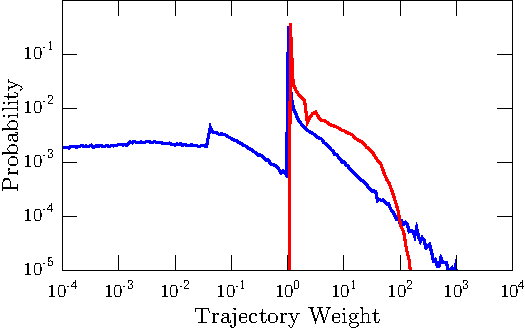
\includegraphics[width=0.8\textwidth]{fig/numerics/TM_normhist}
  \caption[Histogram of Accumulated Numerical TM Estimates]
  {Histogram of accumulated numerical TM estimates, for raw Gaussian (blue) and birth-death Gaussian (red).
    Simulations used $10^6$ paths, with $N=100$ points per path, $\chi=100$, $d=1,T=1.$
  The raw Gaussian distribution extends off to negative infinity, while the birth-death distribution has trunctated peak at zero weight.}
\label{fig:TM_histogram}
\end{figure}

\subsubsection{TM-Gaussian paths}

\begin{figure}
  \centering
  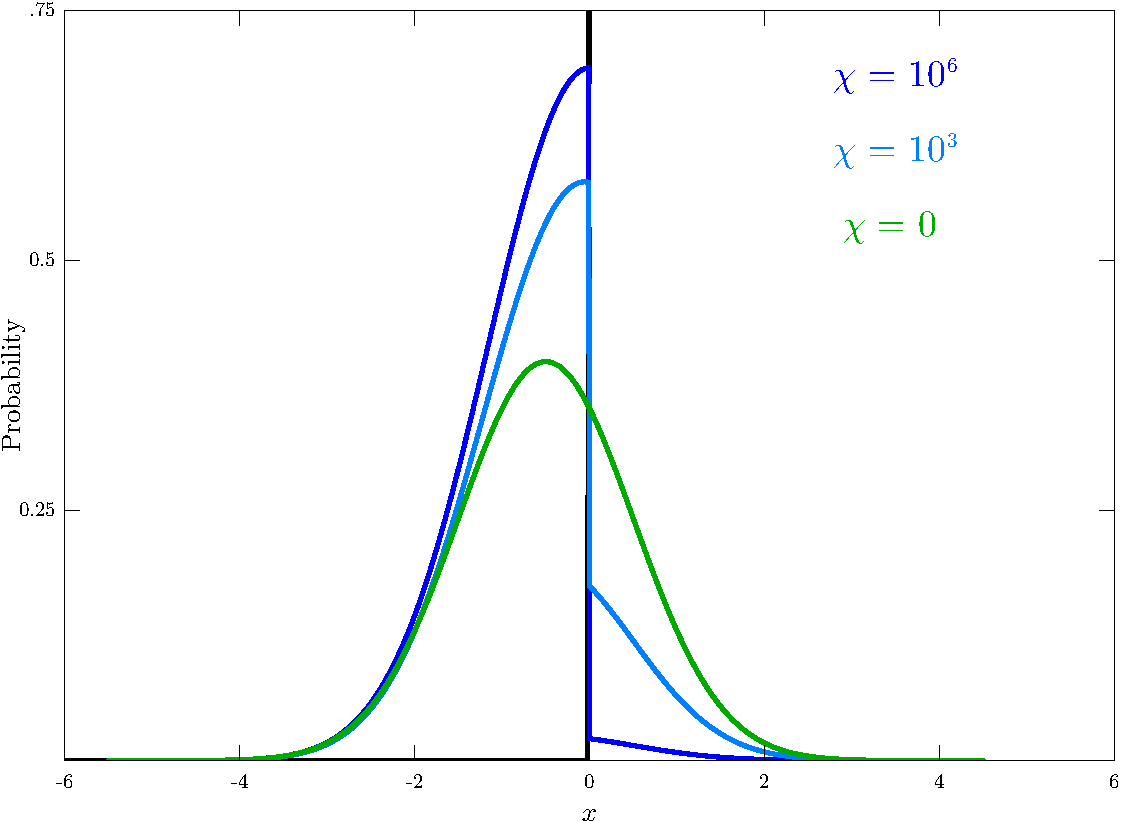
\includegraphics[width=0.8\textwidth]{fig/analytical/probTM}
  \caption[Combined TM Potential and Gaussian probability distribution.]{
    Combined TM-Gaussian probability distribution plotted for various $\chi$.
    Increment starting position is $x=-1$, and $\cT=1$.  The TM boundary is at the origin. }
\end{figure}

One possible solution to the fluctuations is to sample from a combination of a Gaussian
and the path-averaged exponential~(\ref{eq:TM_pot}) for the path increment.
In this case, the total probability distribution for the paths is 
\begin{align}
  P(x_1,\ldots ,x_{N-1}) = \prod_{k=0}^{N-1}\frac{e^{-(x_{k+1}-x_k)^2/(2\Delta\cT)}}{\sqrt{2\pi\Delta\cT}}
  \bigglinklangle e^{-\int_0^{\Delta \cT}dt\, \VTM}\bigglinkrangle_{x_k\rightarrow x_{k+1}}
\end{align}
In the same manner as the v-loops, the Gaussian probability distribution can be decoupled into a
set of random variables, where from Eq.~\ref{eq:open_vloop}, the argument of each of those Gaussians 
involves ${z_k = (x_k-c_{k}x_{k-1})/\sqrt{c_k\Delta \cT}}$.
\begin{align}
  P(x_1,\ldots ,x_{N-1}) = v_{N,N-1}\prod_{k=0}^{N-1}\cN_{k+1}^{-1}P\supTM_{k+1}(x_{k+1}),
\end{align}
where the new probability distribution for $x_k$ is 
\begin{align}
P\supTM_{k+1}(x_{k+1}):=\cN^{-1}_{k+1}\frac{e^{-(x_{k+1}-c_k x_k)^2/(2c_k\Delta\cT)}}{\sqrt{2\pi c_k\Delta\cT}}v_{k,k+1}(x_k,x_{k+1}),
  \end{align}
with normalization constant 
\begin{align}
  \cN_k=\int dy\, \frac{e^{-(y-c_k x_k)^2/(2c_k\Delta\cT)}}{\sqrt{2\pi c_k\Delta\cT}}v_{k,k+1}(x_k,y).
\end{align}
The crucial point is that the $P\supTM_{k}$ can be sampled from, accounting only for the present position. 
While the present position $x_k$ is still coupled to future positions via $v_{k+1,k}$, the sampling procedure ignores
that coupling and samples $x_k$ based solely on $P_k$.  
The probability distribution can be put into a convenient numerical form by completing the square to account
for $v_{k,k+1}$.  The resulting piecewise Gaussian probability distribution is 
\begin{align}
  P\supTM_{k+1}(x_{k+1})
 = \cN_k\left\{ \begin{array}{lc}
     \vspace{0.2cm}  \dfrac{e^{-(x_{k+1}-c_k x_k)^2/(2c_k \Delta\cT)}}{\sqrt{2\pi c_k \Delta\cT}} + \sgn(d-x_k)\dfrac{\tanh\Xi}{\sqrt{2\pi c_k \Delta\cT}} & \hspace{2cm}\\
    \vspace{0.2cm} \hspace{0.7cm}\times e^{-(x_{k+1}-c_k(2d-x_k))^2/(2c_k \Delta\cT)} e^{-2(1-c_k)d(d-x_k)/\Delta\cT} &  X_{k,k+1}>0\\
\dfrac{\sech \Xi}{\sqrt{2\pi c_k \Delta\cT}}e^{-\frac{(x_{k+1}-c_k x_k)^2}{2c_k \Delta\cT}}  &  X_{k,k+1}<0\,,\\
\end{array}
\right.\label{eq:PTM_k}
\end{align}
where we previously defined $X_{k,k+1}=(d-x_k)(d-x_{k+1})$.  
The normalization constant integral can be evaluated in two parts $\cN_k=\cN_k^{\text{C}}+\cN_k^{\text{NC}}$, 
a crossing term $\cN_k^{\text{C}}$ for $X_{k,k+1}<0$,  and non-crossing term $\cN_k^{\text{NC}}$ for $X_{k,k+1}>0$,
 with the result
\begin{align}
  \cN_k^{\text{C}}=\,& \frac{1}{2}\left[1+\sgn(d-x_k)\, \erf\!\left(\frac{d-c_k x_k}{\sqrt{2 c_k \Delta\cT}}\right)\right] \nonumber\\
  &+\sgn(d-x_k) \frac{\tanh\Xi}{2}\left[1+ \sgn(d-x_k)\,\erf\!\left(\frac{d(1-2c_k)+ c_kx_k}{\sqrt{2c_k \Delta\cT}}\right)\right]\nonumber\\
  & \hspace{2cm}\times e^{-2(1-c_k)d(d-x_k)/\Delta\cT} \\
 %  &=\frac{1}{2}\left[1- \erf\left(\frac{d-c_k x_k}{\sqrt{2 c_k \Delta\cT}}\right)\right]
 % - \frac{\tanh\Xi}{2}\left[1- \erf\left(\frac{d(1-2c_k)+ c_kx_k}{\sqrt{2c_k \Delta\cT}}\right)\right]e^{-\frac{2(1-c_k)d(d-x_k)}{\Delta\cT}}\text{d<x_k}.
% \end{align}
% \begin{align}
\cN_k^{\text{NC}}=\,& \frac{\sech\Xi}{2}\left[1-\sgn(d-x_k) \erf\left(\frac{d-c_k x_k}{\sqrt{2 c_k \Delta\cT}}\right)\right].
\end{align}
The probability distribution~(\ref{eq:PTM_k}) can be sampled via the following procedure.
First, note that the probability distributions involve truncated Gaussians in $x_k$.  The truncation
occurs at the surface, since the probability distribution was split based on wether path-increments cross
through the surface or not.
 The truncation ensures that the crossing or no-crossing constraint, $X_{k,k+1}$ is obeyed.  
At each step the simulation picks the crossing or no-crossing branch of the probability distribution
cased on the relative weights of $\cN_k^\text{C}$ and $\cN_k^\text{NC}$, picking the crossing branch 
if $\cN_k^{\text{C}}/\cN_k<r$ where $r$ is a uniform random number.  
If the crossing branch is chosen, then a deviate is sampled from the truncated Gaussian distribution.
If the no-crossing branch is chosen, then depending on the sign of $\sgn(d-x_k)$, there are another two options.
If $\sgn(d-x_k)>1$, then one of the Gaussians is picked based on their relative probability of occuring,
and a deviate is sampled from one of them.
If however, $\sgn(d-x_k)<1,$ then the rejection method is used to generate a deviate.
In the rejection method, a deviate is sampled from a proposal distribution $P_1(x)$(such as one of the Gaussians),
and accepted with a probability $P_2(x)/P_1(x)$, where  $P_2$ is the target distribution~\cite{NumRecipe}.
In the other cases, the truncated Gaussian distributions can be sampled quickly via the inverse error function.  

While this method does improve performance, it still relies on taking a product of $N-1$ normalization factors $\cN_k$,
where $0<\cN_k<2$.  This leads to the same problems with numerical fluctuations as the plain Gaussians
as the path length $N$ is increased.  It is also much more involved to implement than the plain Gaussian
approach.

\subsubsection{Birth-Death Loop Swarm}

Both the plain Gaussian and TM-Gaussian paths can be rescued by further adjusting the sampling procedure.
In both cases, as the trajectory propagates it accumulates a large weight.  After $k$ steps,
the weight is $w_k=\prod_{j=1}^k\nu_j$, where $\nu_j$ represents either $v_{j,j+1}$ for Gaussians or $\cN_j$
for the TM-Gaussians.  Most paths propagating around the interface will acquire 
a number of large weights with $\nu_j>1$ from the vacuum side, 
and small weights $0<\nu_j<1$ from within the medium.  
The logarithm of the accumulated weight is $\log w_k = \sum_{j=1}^k\log \nu_j$.  
Since the $\nu_j$ are random variables (since both the $v_{k,k+1}$ and $\cN_k$ are functions of an underlying random path),
then we would expect $\log w_k$ to be normally distributed, with some variance $\sigma$. 
Thus, the accumulated weight is expected to grow a log-normal deviate, with variance $\sigma^N$.    
Note that the mean would still have the correct value, but the variance, and thus sampling error would
grow unacceptably as $N$ increases.

A large number of paths will yield very low values, and a lot of computer time would be wasted on simulations
which computing numbers very close to zero.  A few rare paths would skirt outside the surface, accumulating
very large weights, and contributing a lot to the Casimir energy.  Together these lead to large statistical
fluctuations, which make it hard to get sufficient averaging for even moderately fine paths $N\sim 100$.
Note that both types of paths will contribute to the Casimir energy.

The path generation for either method can be modified as follows.  The weight $w_k$ is effectively treated as 
the fitness function for the path.  Paths with high weights will spawn further paths (birth), while paths with
small weights will be terminated and return zero (death).
If the weight is becoming small, $w_k<0.5$ then compare $w_k$ with a uniform random number $u$.
If $w_k<u$, then set $w_k=0$ and stop propagating the path; alternatively, if $w_k>u$, then 
the path survives and the weight is reset $w_k=1$.  That is the death process.
In an ensemble average, an average fraction of the paths $u$ survive the death process, which gives 
the correct average value.
If the weight is becoming large, $w_k>2$, then split the weight in half, and assign each half to 
two independent trajectories.
Altogether, this is called the birth-death process, and should be applied at every step of the random path.
Implementing the deaths ensures that the memory requirements do not grow exponentially as a function 
of path length, while the birth process ensures that successful trajectories with a large weight have 
more opportunity.  Note that returning zero is still a contribution to the Casimir energy (anything different
from unity will contribute), and the death process speeds up the computation by not computing ever smaller
values.

The birth-death process is a very simple Markov Chain Monte Carlo (MCMC) method.  The birth-death
process modifies the preferred motions based on the accumulated weight.  Paths are likely to be born
on the vacuum side of interfaces, and they are likely to die on the inside of the interface.
Far away from the interface on either side, the paths are unlikely to change.  

Similar, but different terms are discussed throughout stochastic processes literature.
The more typical birth-death process is used in queuing theory, where 
the number of objects in a queue randomly increases and decreases at a fixed average rate.
In our case, that rate depends on the past behaviour of the system, and where it has gone.  
The process used here is closer to the genealogical methods for evaluating path integrals discussed by Del Moral~\cite{DelMoral2004}.
A similar genealogical idea has been used in quantum trajectory simulations~\cite{Jacobs2010a}, which is another
technique for simulating open quantum systems.  In that variant, each random trajectory carries 
a probability weight.  If that weight becomes too small, then that random trajectory is killed,
and another more successful trajectory is split in two, and given half the weight.   
A similar method has been used to discuss simulating rare events, such as the extreme tails of a Gaussian.
In that case, one splits trajectories based on whether they exceed a certain threshold criterion~\cite{Glasserman1999,Garvels2000}.
These methods essentially reward the trajectories or paths of the system that enter regions with a large
contribution to the integral (or other figure of merit).  

\begin{figure}
  \centering
  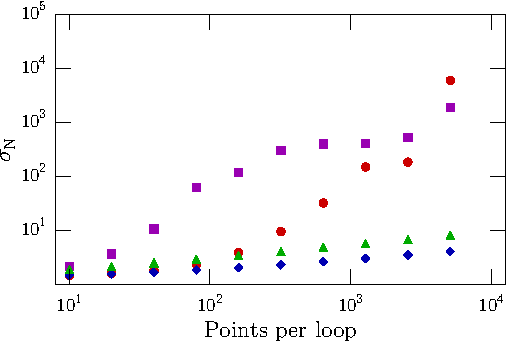
\includegraphics[width=0.8\textwidth]{fig/temp/TM_scalingN}
  \caption[Scaling of variance TM potential as function of $N$ for four methods.]
  {Scaling of variance TM potential as function of $N$ for four methods.  
  All combinations of Gaussian paths increments and combined TM-Gaussian steps, with raw values and 
  birth-death.}
\label{fig:TM_scalingN}
\end{figure}

Fig.~\ref{fig:TM_scalingN} shows how the Gaussian and TM-Gaussians estimates of the simple path integral
scale with the path resolution.  The birth-death process has been applied to both ways of generating paths.
The birth-death process reduces the variance, and makes both methods much more tractable.
The difference between Gaussian and TM-gaussians is small under the birth-death process.
Given that small difference, and the relative simplicity of the Gaussians, we have opted to 
use the birth-death process in conjunction with Gaussians throughout the remainder. 

\subsection{Monte-Carlo Sampling for Path-Time}

\label{sec:expT-sampling}

The TM polarization requires a slightly different sampling method for generating path-times $\cT$.  
In some limited cases it may be possible to estimate a minimum $\cT_0$ where 
the integrand is small for a given path, and a path is unlikely to have branched or birthed new paths.  
For paths starting on the vacuum side near a dielectric, the accumulated
potential at small path-times is approximately ${\prod_k( 1+\tanh\Xi e^{-2(d-x_k)(d-x_{k+1})/\Delta\cT})}$,  
which turns on smoothly in $\cT$.
In that case, $\cT_0$ can be estimated from the time an initial, fiducial path would contact a surface and the 
integrand would turn on.  The path-time can be sampled from the power law distribution~(\ref{eq:Tpower_law}).
The birth-death process then proceeds starting with the initial path.  

However, in a two-body geometry that sort of estimation fails.
The renormalized integrand is only nonzero for paths that come close to both surfaces.
Since the birth-death method may split the trajectory, it is not always possible to reliably
find a minimum time $\cT_0$ when the renormalized integrand turns on.  (A very small $\cT_0$ could be picked, 
where the path has no chance of touching the surface, but most computations would return zero,
 since the most probable $\cT$ are close to $\cT_0$.)
As a result, it is not possible to estimate for a single trajectory a lower bound $\cT_0$ 
for which the path does not branch, but is also close to when the integrand turns on.  

Since the birth-death method essentially enlarges the ensemble of paths selected, it's turn on
closely mimics the probability for a Brownian bridge to touch a surface.  The probability for 
a Brownian bridge to touch a surface a distance $d$ away in path-time $\cT$ is 
\begin{equation}
  P_{\text{touch}}(\cT) = e^{-2d^2/\cT}.
\end{equation} 
The combined potential term ${\prod_kv_{k,k+1}$,  also has a similar dependence.  
This could be combined with the $\cT^{-(1+D/2)}$ power law for a new probability distribution.  
\begin{equation}
  P_{\text{exp-T}}(\cT;\cT_0,s) = \frac{\cT_0^{s-1}}{\Gamma[s-1] \cT^s}e^{-\cT_0/\cT}\label{eq:expT},
\end{equation}
where $s>1$ and $\cT_0>0$.  For the Casimir energy at zero temperature, $s=1+D/2$.  But for estimating
thermal Casimir energies or forces, that power $s$ may change.  
%  The exponential factor effectively models the finite touching 
% probability for Brownian bridges starting at the origin to touch a planar surface a distance $d$ 
% away in time $\cT$, $P_\text{touch}=e^{-2d^2/\cT}$. 

The probability distribution~\ref{eq:expT} can be transformed to $u=\cT_0/\cT$, for 
which the probability distribution is
\begin{equation}
  P_{\text{exp}-1/\cT}(u;\cT0,s) = \frac{u^{s-2}}{\Gamma[s-1]}e^{-u}.
\end{equation}
% where we had to include $du/d\cT= -(\cT_0)/\cT^2=-1/(\cT_0u^2)$ for the change
% of measure.  
The new variable $u=\cT_0/\cT$ has the form of a Gamma distribution, which has probability density 
\begin{equation}
  f(x) = \frac{x^{a-1} e^{-x/b}}{\Gamma(a)b^a}.  
\end{equation}
where $a>0$ and $b>0$ are the shape and scale parameters respectively~\cite{Devroye2003}.  
For small integer or half-integer powers $a$, there are some simple methods for generating 
gamma deviates $g_i$.  
A sum of Gamma deviates $\sum_{i=1}g_i$ with shape parameters $a_i$, is also a Gamma deviate
with shape parameter $\sum a_i$~(see pg. 402 of Devroye~\cite{Devroye2003}).  
In particular, this means the sum of $k$ exponential deviates $e_i=-\log(u_i)$, yields a Gamma 
deviate gamma(k,1).  Furthermore if $z$ is normally distributed then $z^2/2$ obeys gamma$\left(\frac{1}{2},1\right)$.
For small integer powers, $\cT$ is distributed according to
\begin{equation}
  \cT\sim \frac{\cT_0}{-\sum_{i=1}^{s}\log u_i},
\end{equation}
while for half-integer powers, 
\begin{equation}
  \cT\sim \frac{\cT_0}{-\sum_{i=1}^{\text{floor}(s)}\log u_i+z^2/2}.
\end{equation}
The integer powers are useful for estimating zero temperature Casimir energies. The half-integer powers
naturally emerge when considering the thermal Casimir energy, or derivatives of the Casimir energy 
such as the force.  
This distribution can also be used to sample times $\cT$
even for TE integrands.  In that case however, it is possible the generated path will not
touch all bodies and merely return zero.    

\section{Gradient Estimation}

\begin{enumerate}
  \item Need gradients to compute forces, torques from potential.  Also need it directly
    for TM Casimir-Polder energy.
  \item Looking for corrections to gravity need curvature.  Similarly, estimating 
    (Cite Cornell expt) change in oscillation frequency.  Need two spatial derivatives.
    For TM potential, this is 4 spatial derivatives.  
\end{enumerate}

    \begin{enumerate}
      \item Need gradient estimation.  Use Malliavin calculus~\cite{Fournie1999, Chen2007,Kohatsu-Higa2003}.
        Formal introductions \cite{Nualart2006, Malliavin2006, DiNunno2009}.
      \item Birth-death methods to handle product of increments.  Related to Genealogical 
        methods used in rare-event simulation.  
    \end{enumerate}

Let us consider the sensitivity of an expectation value $\dlangle f \drangle = \int dx f(x)P(x)$,
with respect to a parameter $\Theta$, where $P(x)$ is the probability distribution.  
    The likelihood ratio method relies on differentiating the underlying probability distribution,
    and evaluating $\partial_\Theta\dlangle f\drangle=\dlangle f(x)\partial_\Theta\log P(x;\Theta)\drangle$.  
    One can then estimate the gradient by generating 
    samples using the original probability distribution, while evaluating this new function.
    This can be readily applied to computing sensitivities of expectations with respect to Brownian motion~\cite{Broadie1996}.  
    A similar idea exploits the Malliavin calculus~\cite{Nualart2006}:
    In the Malliavin framework, one can estimate a sensitivity by evaluating $\dlangle f(x)\pi_\Theta(x)\drangle$,
    where $\pi_\Theta$ is the Malliavin weight~\cite{Fournie1999}.  
    The Malliavin calculus is essentially functional differentiation with respect to the Brownian motion.  
    One can derive the Malliavin weights by exchanging derivatives with respect to the parameter for
    derivatives with respect to the Brownian motion, and integrating by parts~\cite{Kohatsu-Higa2004}.  
    The Malliavin results can be recovered for Brownian motion if one combines the likelihood-ratio method with partial-averaging
    along the Brownian motion~\cite{Chen2007}.  In either case, one exchanges differentiation for
    evaluating a new reweighted function, which depends on the required derivatives, while still
    using the original paths.  


\subsection{Finite Differences}

\begin{enumerate}
  \item Simple to implement.  However, larger fluctuations, and biased. 
  \item Best to use common random numbers.  Also provides better error estimate.
  \item Need to balance choosing $N$, $ds$.  
  \item However difference-of-ensembles has better behaviour than 
    ensemble-of-differences.  Some ordering of operations noticeably superior.  
    Essentially passes finite difference onto $1/\cT^3$, which is nice and smooth.
\end{enumerate}

\subsection{Partial Averaging-Gaussian Paths}

\label{sec:partial_average}
\begin{enumerate}
  \item Consider how to evaluate Gradients with respect to source point of Gaussian 
    path integrals of the energy $\epsr$
    \begin{align}
      E =& -\frac{\hbar c\alpha_0}{2(2\pi)^{D/2}}\int \frac{d\cT}{\cT^{1+D/2-\alpha}}
      \biggdlangle \frac{1}{\langle\epsr\rangle}\biggdrangle\\
      =& -\frac{\hbar c\alpha_0}{2(2\pi)^{D/2}}\int \frac{d\cT}{\cT^{1+D/2-\alpha}}\int ds\,\frac{s^{\alpha-1}}{\Gamma[\alpha]}
      \biggdlangle e^{-s\cT \langle \epsr\rangle}\biggdrangle
    \end{align}
  \item If we use unshifted integration variables, $\vect{x}_k$, rather than the shifted, scaled
    Brownian motion variables, can differentiate immediately.
    Momentarily focus on just the path integral piece,
    \begin{equation}
      P = \biggdlangle e^{-s\cT \langle \epsr\rangle}\biggdrangle 
      = \int \prod_{j=1}^{N-1}dx_k \prod_{j=0}^{N-1}\frac{1}{(2\pi \Delta T)^{D/2}}e^{-(\vect{x}_{j+1}-\vect{x}_j)^2/2\Delta T-s\Delta T \epsr(\vect{x}_j)}.
    \end{equation}
    Main component are derivatives w.r.t. Gaussian.  Will neglect derivatives of the potential.  
    Our basic idea is to integrate out intermediate coordinates.  Under the assumption the 
    the integrands are approximately stable, or that the steps compose, we can average multiple
    steps.
  \item This is related to choosing a non-uniform loop with less resolution close to the beginning of the 
    loop.  This is justified via switching integration and differentation.  The Gaussian integrals 
    obviously compose.  The derivatives can just be carried out at the very end.  
  \item Derivatives of the Gaussian are Hermite polynomials:
    \begin{equation}
      \frac{d^n}{dx^n} e^{-x^2} = (-1)^n H_n(x)e^{-x^2}
    \end{equation}
    Scaling the variables to $x\rightarrow x/a$ yields
    \begin{equation}
      \frac{d^n}{dx^n} e^{-(x-\mu)^2/a^2} = a^{-n}(-1)^n H_n\big(\frac{x-\mu}{a}\big)e^{-(x-\mu)^2/a^2}
    \end{equation}

    \item The simplest approach is to exchange integration and differentiation, then completing the square in $x_0$,
    and then carry out the derivatives
    \begin{align}
      C=&\partial_0^n\int dx_1  \frac{1}{(2\pi)^{3/2}\sqrt{T_1T_2T_{N_1}}}e^{-(x_0-x_1)^2/(2T_1)-(x_1-x_2)^2/(2T_2)-(x_0-x_{N-1})^2/(2T_{N-1})}\\
%      =&\partial_0^n \frac{1}{2\pi\sqrt{(T_1+T_2)T_{N_1}}}e^{-(x_0-x_2)^2/[2(T_1+T_2)]-(x_0-x_{N-1})^2/(2T_{N-1})}\\
      =&\partial_0^n \frac{1}{2\pi\sqrt{(T_1+T_2)T_{N_1}}}e^{-(x_0-\mu_2)^2/[2\sigma_2^2]-(x_2-x_{N-1})^2/(2[T_{N-1}+T_1+T_2])}\\
      =&(-1)^n(\sqrt{2}\sigma_2)^{-n/2}H_n\bigg(\frac{x_0-\mu_2}{\sqrt{2}\sigma_2}\bigg)
      \frac{1}{(2\pi)\sqrt{(T_1+T_2)T_{N_1}}}\nonumber\\
      &\times e^{-(x_0-x_2)^2/[2(T_1+T_2)]-(x_0-x_{N-1})^2/(2T_{N-1})},
    \end{align}
    where 
    \begin{gather}
      \mu_2 = \frac{T_{N-1}x_2+ (T_1+T_2)x_{N-1}}{T_1+T_2+T_{N-1}}\\
      \sigma_2^2 = \frac{(T_1+T_2)T_{N-1}}{T_{N-1}+T_1+T_2}
    \end{gather}
  \item Now evidently if we integrate out points symmetrically from the loop origin, and we 
    assume all $T_i=\Delta T$, then after integrated out $m$ steps we have 
    \begin{gather}
      \bar{x}_m = \frac{x_{m+1}+ x_{N-m-1}}{2}\\
      \sigma_2^2 = m\Delta T.
    \end{gather}
    The gradient of the path integral can then be approximately written as 
    \begin{align}
      C\approx
      &(-1)^n(\sqrt{2 T_m})^{-n/2}H_n\bigg(\frac{x_0-\bar{x}_m}{\sqrt{2 T_m}}\bigg)\nonumber\\
      &\times \frac{1}{(2\pi T_m)}e^{-(x_0-x_{m+1})^2/(2T_m)-(x_0-x_{N-m-1})^2/(2T_m)}.
    \end{align}
  \item We can estimate how many steps to integrate out based on the touching probability in time $T_m$.  
    The probability to touch a plane a distance $d$ away in time $T_m=m\Delta T = (m/N)T$ is 
    \begin{equation}
      P_{\text{touch}} = e^{-2d^2/T_m},
    \end{equation}
    which can be solved for $m$ if we require that $P_{\mathrm{touch}}$ does not exceed a threshold
    $10^{-\rho}$ with $\rho>0$  
    \begin{equation}
      \frac{m}{N} \le \frac{2d^2}{T\rho\ln(10)}.
    \end{equation}
    Note that as $N$ increases, the integration point approaches a constant fraction, even as $N$ increases.  
    This in effect reduces the fluctuations by $m^n$.  
    \item This is in effect choosing to make a loop with non-uniform steps, where in particular the first
    and last step are larger than the others.  We choose the size of those steps to be as 
    large as possible, while not interacting much with a the nearest surface.  

    \item Problem with adaptive choice?
\end{enumerate}

\subsection{General Method Near Surfaces}

     While estimating gradients for the stress-tensor it may be necessary to estimate 
    gradients while close to one surface.  For a renormalized energy, only loops that touch both
    surfaces will contribute.   In this case, the above approach based on integrating out Gaussians
    is of limited utility in reducing the fluctuations.  The assumption that the integrals are approximately
    Gaussian can only be explited for a very small number of steps.  
    However, if we assume there is a Feynman-Kac formula available taking into account the 
    interaction with a simple surface, then similar reasoning can be used.  In this case
    one integrates out further steps, since the Feynman-Kac formulae compose with one another,
    where now the threshold is must balance the path wandering sufficiently far that a simple 
    approximation.

    For example, consider using the Feynman-Kac formula for open loops near a Dirichlet surface, 
    \begin{equation}
      \dlangle e^{-V_D(x-d)}\drangle_{x_{j}\rightarrow x_{j+1}} 
      = \Theta[(x_j-d)(x_{j+1}-d)]\left(1-e^{-2(x_j-d)(x_{j+1}-d)/T}\right)
    \end{equation}

\begin{enumerate}
  \item Gradients for atom
  \item Stress energy tensor 
\item Application to stress-tensor.  (Evaluate derivatives first, then take limit.)
  Problematic for stress-tensor values near one surface in 2-body scenarios. (Use exponential expressions
  to allow non-Gaussian integration.  Must just be stable distribution  
  Thus expact larger fluctuations near surfaces.  
  For example, stress-energy tensor requires 
  \begin{equation}
   T_{zz}=\lim_{\Delta\rightarrow 0} [\partial_{x_{CP}}^2 - \partial_{\Delta}^2]\dlangle \mathfrak{M}\drangle,
  \end{equation}
  where $\Delta = (x_N-x_0)/2, x_{CP} = (x_N+x_0)/2$.  Using the chain-rule, and employing the
  same differentiation this becomes. where $x_{CP}$ is the centre-point, and $\Delta$ is the separation.
%   \begin{gather}
%     x_{CP} =  \frac{1}{2}(x_{N}+x_0)\\
%     \Delta = \frac{1}{2}(x_{N}-x_0)\\
%     x_0  = x_{CP}-\Delta\\
%     x_N = x_{CP}+\Delta
%   \end{gather}
%   Then
%   \begin{align}
%     \frac{\partial}{\partial x_{CP}} 
%     %&= \frac{\partial x_0}{\partial x_{CP}}\frac{\partial}{\partial x_0}
%     % +\frac{\partial x_N}{\partial x_{CP}}\frac{\partial}{\partial x_N}\\
% &= \frac{1}{2}\frac{\partial}{\partial x_N}+\frac{1}{2}\frac{\partial}{\partial x_0}\\
%   \frac{\partial}{\partial \Delta} 
% %&= \frac{\partial x_0}{\partial \Delta }\frac{\partial}{\partial x_0}
% %    +\frac{\partial x_N}{\partial \Delta}\frac{\partial}{\partial x_N}\\
% &= \frac{1}{2}\frac{\partial}{\partial x_N}-\frac{1}{2}\frac{\partial}{\partial x_0}
%   \end{align}
Then expanding these derivatives out (correct expression?)
\begin{align}
  T_{zz} &= \lim_{x_N\rightarrow x_0}\frac{1}{4}[(\partial_0+\partial_N)^2+(\partial_0+\partial_N)^2]G\\
  &= \lim_{x_N\rightarrow x_0}\frac{1}{2}[\partial_0^2+\partial_N^2]G
\end{align}

\end{enumerate}

\subsection{Hermite-Gaussian Sampling}

In order to apply the Hermite-Gaussian method to high order derivatives, it is best to 
sample from the combined Hermite-Gaussian.  The simplest approach uses Gaussian samples, weighted
by the appropriate Hermite-Gaussian function.  While this is acceptable for the first or second derivatives,
it breaks down for higher derivatives.  In particular, the Gaussian samples are most likely to be in a narrow
range $x\in(-3\sigma,3\sigma)$.  The Hermite-Gaussian oscillates in sign in this range, and
the dominant contributions come from the tails $x\sim \sqrt{n}\sigma$.  So for a finite sample,
one would see large fluctuations.  

The combined Gaussian steps for both $x_1, x_2$ which are pinned to start at $x_0$ is 
\begin{align}
  G &= \frac{1}{2\pi T_1T_2}\exp\left[-\frac{(x_0-x_1)^2}{2T_1}-\frac{(x_0-x_2)^2}{2T_2}\right]\\
  % &= \frac{1}{2\pi T_1T_2}\exp\left[-\frac{T_1+T_2}{2T_1T_2}x_0^2 +\left(\frac{x_1}{T_1}+\frac{x_2}{T_2}\right)x_0
  %   -\frac{x_1^2}{2T_1}-\frac{x_2^2}{2T_2}\right]\\
  &= \frac{1}{2\pi T_1T_2}\exp\left[-\frac{T_1+T_2}{2T_1T_2}\left(x_0 -\frac{x_1T_2+T_1x_2}{T_1+T_2}\right)^2
    -\frac{(x_1-x_2)^2}{2(T_1+T_2)}\right]
\end{align}
After differentiation w.r.t $x_0$, one finds 
\begin{equation}
  HG:= \partial_0^n G 
= \frac{1}{\sqrt{2\pi\sigma^2}\sqrt{2\pi(T_1+T_2)}} 
(-1)^n(2\sigma^2)^{-n/2}H_n\left(\frac{x_0-\mu_H}{\sqrt{2\sigma_H^2}} \right)
  \exp\left[-\frac{(x_0-\mu_H)^2}{2\sigma_H^2} - \frac{(x_1-x_2)^2}{2(T_1+T_2)}\right],
\end{equation}
where 
\begin{gather}
  \sigma_H^2:= \frac{T_1T_2}{(T_1+T_2)}\qquad
  \mu_H := \frac{x_1T_2+T_1x_2}{T_1+T_2}.
\end{gather}
In the event that $T_1=T_2$, this simplifies down to 
\begin{gather}
  \sigma_H^2:= \frac{T_1}{2}\qquad
  \mu_H := \frac{x_1+x_2}{2}.
\end{gather}
In order to make samples that are useful for closed paths one must include 
the normalization factor for the ``open'' Gaussian bridge that connects the end points $x_1$ and $x_2$
in time $T-T_1-T_2$.  
The total distribution for $x_1,x_2$ is 
\begin{align}
  HG'(x_1,x_2)&:=\frac{1}{\sqrt{2\pi\sigma^2}\sqrt{2\pi(T_1+T_2)}\sqrt{2\pi(T-T_1-T_2)} }
  (2\sigma^2)^{-n/2}H_n\left(\frac{x_0-\mu}{\sqrt{2\sigma^2}} \right)\nonumber\\
  &\hspace{0.5cm}\times\exp\left[-\frac{(x_0-\mu)^2}{2\sigma^2} - \frac{T(x_1-x_2)^2}{2(T-T_1-T_2)(T_1+T_2)}\right],
\end{align}
However, this is not normalized, and can even change sign.  
The samples must be taken from the absolute value of the integrand, with the sign of the Hermite-Gaussian
function weighting the samples.
The sign changes will naturally lead to cancellation.  In the presence of a potential $\Phi[x(t)]$,
the cancellation is not perfect and the result is non-zero.  
In order to best carry out the cancellation, and reduce fluctuations one should pair each sample of 
the Hermite-Gaussian with its negative.  

The probability distribution for the combined steps can be most naturally formulated in terms of the decoupled variables
\begin{align}
  \bar{x}:=\frac{x_1+x_2}{2}\\
  \Delta x := x_2-x_1.
\end{align}
The probability distributions for $\bar{x}$ and $\Delta x$ decouple as 
\begin{align}
  P_{HG,1}(\bar{x})&:=\frac{1}{\sqrt{2\pi\sigma_H^2}} 
  \bigg|H_n\bigg(\frac{x_0-\bar{x}}{\sqrt{2\sigma_H^2}} \bigg)\bigg|
  %\nonumber\\  &\hspace{0.5cm}\times
  \exp\left[-\frac{(x_0-\bar{x})^2}{2\sigma_H^2}\right]\\
  P_{HG,2}(\Delta x) &:=\sqrt{\frac{T}{2\pi(T_1+T_2)(T-T_1-T_2)}}
%  &\hspace{0.5cm}\times
\exp\left[- \frac{T(x_1-x_2)^2}{2(T-T_1-T_2)(T_1+T_2)}\right],
\end{align}
The numerical average can be computed as 
\begin{equation}
  I = \dlangle (-1)^n(2\sigma_H^2)^{-n/2}\eta_Hs_Hf\drangle_{HG},
\end{equation}
where $x_1,x_2$ are sampled from $P_{HG}$, and the remaining sub-bridge is sampled via
the open Gaussian probability distribution.  
where the normalization $\eta_H$ and sign factor $s_H$ are defined as 
\begin{align}
  s_H &:= \sgn\bigg[H_n\left(\frac{x_0-\mu_H}{\sqrt{2\sigma_H^2}} \right)\bigg] \\
  \eta_H &:=\frac{1}{\sqrt{2\pi T}}\int dy \frac{1}{\sqrt{2\pi\sigma_H^2}}
  \big|H_n\left(\frac{x_0-y}{\sqrt{2\sigma_H^2}} \right)\big|
%  \nonumber\\  &\hspace{0.5cm}\times
\exp\left[-\frac{(x_0-y)^2}{2\sigma_H^2}\right],
\end{align}

It is best to numerically sample from distributions with unit variance, and rescale the deviates 
by the time.  In which case, $\bar{x}=h\sqrt{2\sigma_H}$, and $\Delta x = \sqrt{2T_1(T-2T_1)/T}z$,
where $z$ is a standard normal deviate as $h$ is sampled from 
\begin{align}
  P'_{HG,1}(h)&:=\frac{1}{\eta'_H\sqrt{\pi} }  \bigg|H_n\bigg(-h\bigg)\bigg|e^{-h^2}\\
  \eta'_H&=:=\int dh P'_{HG,1}(h).
\end{align}

The raw deviates will be denoted $h$ and $z$.% , where 
% \begin{align}
%   \frac{1}{2}(x_1+x_2) &= x_0 + \sqrt{\frac{T_1}{2}}h\\
%   -x_1+x_2 &= \sqrt{\frac{2T_1(T-2T_1)}{T}}z
% \end{align}
Then solving for $x_1, x_2$, 
\begin{align}
  x_1 & = x_0 + \left(\sqrt{\frac{T_1}{2}}h-\sqrt{\frac{T_1(T-2T_1)}{2T}}z\right)\\
  x_2 & = x_0 + \left(\sqrt{\frac{T_1}{2}}h+\sqrt{\frac{T_1(T-2T_1)}{2T}}z\right)
\end{align}
where $h' := h\sqrt{T_1/2}, z' := z\sqrt{\frac{T_1(T-2T_1)}{2T}}$.
\comment{Note these variables are scaled to agree with Dan, whose code seems to output 
  $h/\sqrt{2}$ naturally.  Again, he is treating $H_n(x)e^{-x^2}$ as the probability
  distribution.}






\subsection{TM Numerical Results: Planar Casimir Energies}


\begin{figure}
\centering
  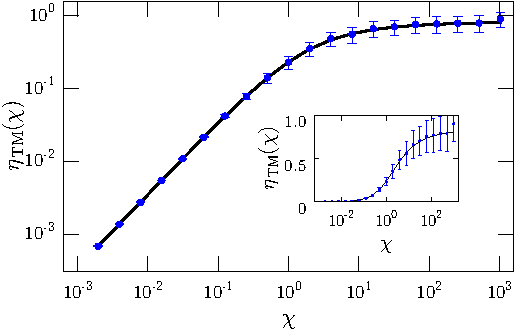
\includegraphics[width=0.8\textwidth]{fig/temp/eff_TM_atom_wall}
  \caption{Numericall computed TM Casimir--Polder Efficiency for Atom-Plane.  }
\end{figure}

\begin{figure}
\centering
  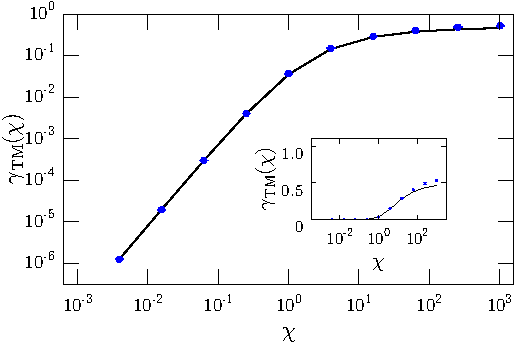
\includegraphics[width=0.8\textwidth]{fig/temp/eff_TM_2wall}
  \caption{Numericall computed TM Casimir Efficiency for Plane-Plane.  }
\end{figure}


\section{Gradients for Casimir Forces and Torques}
\subsection{Surface Pinned Paths}
\label{sec:path-pinning}

\begin{align}
  W &:= \int d\vect{x}_0
  \,\biggdlangle \frac{1}{\langle\epsr\rangle^\alpha}-\frac{1}{[\epsr(\vect{x}_0)]^\alpha}\biggdrangle_{\vect{x}(t)},
  \label{eq:spatial_path_integral}
\end{align}

\begin{equation}
  E = \frac{\hbar c}{2(2\pi)^{D/2}}\int_0^\infty \frac{d\cT}{\cT^{1+D/2}}
  \, W,
  \label{eq:spatial_path_integralE}
\end{equation}

\subsubsection{Force}
The force on a body follows from the gradient of the Casimir energy,
where the derivatives are taken with respect to the body's 
position.
For example, the components of the force on body $2$, expressed
in the basis $\hat{r}_i$, are
given by directional derivatives of the path integral in Eqs.~(\ref{eq:spatial_path_integral}) and 
(\ref{eq:spatial_path_integralE}) with respect to
the components of the body position $\mathbf{R}_2$:
\begin{align}
  &F_{2,i}:=-\frac{\hbar c}{2(2\pi)^{D/2}}\int_0^\infty \!\!\frac{d\cT}{\cT^{1+D/2}}\change{\hat{r}_i\cdot\nablaR2} W
  \nonumber\\
   &\hspace{0.cm}=
   -\frac{\alpha\chi_2\hbar c}{2(2\pi)^{D/2}}
   \hat{r}_i\cdot\!\!
   \int_0^\infty \!\!\!\frac{d\cT}{\cT^{1+D/2}}   \!\int \!d\vect{x}_0\, 
  \Biggdlangle \frac{
  \big\langle 
  \delta(\sigma_2)\,\nabla\sigma_2\big\rangle}
  {\langle\epsr\rangle^{\alpha+1}}\Biggdrangle_{\!\vect{x}(t)}\!\!\!\!,
  \label{eq:forcepathint}
\end{align}
where $\sigma_2 = \sigma_2[\vect{x}(t)-\vect{R}_2]$ in this expression
\change{, and $\nablaR{i}$ denotes the gradient with
respect $\vect{R}_i$.}
The path integration can be simplified by viewing the $\delta$-function,
whose argument involves $\vect{x}(t)$, as a constraint on the
source point $\vect{x}_0$ of the paths.
Writing out the relevant part of the path integral (\ref{eq:forcepathint}),
the $\delta$-function reduces the $D$-dimensional integration
over $\vect{x}_0$ to a $(D-1)$-dimensional integration over
the surface of body 2:
\comment{futzed with this - tried to restore}
\begin{align}
  &\int d\vect{x}_0  \Biggdlangle \frac{
  \big\langle 
  \delta\big(\sigma_2[\vect{x}(t)-\vect{R}_2]\big)\,\nabla\sigma_2[\vect{x}(t)-\vect{R}_2]\big\rangle}
  {\langle\epsr\rangle^{\alpha+1}}\Biggdrangle_{\vect{x}(t)} \nonumber\\
  &\hspace{0.5cm}= 
  \int d\vect{x}_0  \Biggdlangle \frac{
  \delta\big(\sigma_2[\vect{x}_0-\vect{R}_2]\big)\,\nabla\sigma_2[\x0-\vect{R}_2]}
  {\langle\epsr\rangle^{\alpha+1}}\Biggdrangle_{\vect{x}(t)} \nonumber\\
  &\hspace{0.5cm}= 
  \oint_{\sigma_2(\vect{x}_0-\vect{R}_2)=0}^{}
   \hspace{-8ex}dS\hspace{5ex}\biggdlangle 
  \frac{\nabla\sigma_2(\x0-\vect{R}_2)}
  {\langle\epsr\rangle^{\alpha+1}|\nabla\sigma_2(\x0-\vect{R}_2)|}\biggdrangle_{\vect{x}(t)},
  \label{eq:delta-normal}
\end{align}
where the final integral (over path source points $\vect{x}_0$)
is a surface integral over the 
surface of body 2.  The first equality here can be understood
in terms of a discrete path (i.e., in a ``time-slicing'' regularization
of the path integral), where the path average in the numerator
amounts to a sum of terms, each involving a $\delta$-function
involving a path coordinate $\vect{x}_j$.  In the average over all
paths and sum over all source points $\vect{x}_0$,
the $\delta$-function is equivalently a function of the
source point, since $\vect{x}_j$ is the source point
of another equivalent path.
The second equality of Eqs~(\ref{eq:delta-normal})
follows from an application of the H\"ormander formula
(see Eq.~(22) in Ref.~\cite{Mackrory2016}).
The renormalized force vector can be found by summing over all force components and subtracting 
the corresponding single-body energy,
\change{used ``limit'' on oint to get limits underneath integral}
\begin{align}
  \vect{F}_{2}&=
  -\frac{\alpha\chi_2\hbar c}{2(2\pi)^{D/2}}
\int\limits_0^\infty \!\frac{d\cT}{\cT^{1+D/2}}    
\hspace{-3ex}
 \oint\limits_{\sigma_2(\vect{x}_0-\vect{R}_2)=0}^{}
  \hspace{-4ex} dS\hspace{1ex} 
  \hat{n}_2(\vect{x}_0) % \nonumber\\
  % &\hspace{0.5cm}\times 
  \Biggdlangle\frac{1}{\langle\epsilon_{\mathrm{r},12}\rangle^{\alpha+1}}-\frac{1}{\langle\epsilon_{\mathrm{r},2}\rangle^{\alpha+1}}
  \Biggdrangle_{\vect{x}(t)},
  \label{eq:pinning_force}
\end{align}
where the unit-normal vector for the surface of body 2 is defined by
\begin{equation}
  \hat{n}_2(\x0) := -\frac{\nabla \sigma_2(\x0-\vect{R}_2)}{|\nabla \sigma_2(\x0-\vect{R}_2)|}.
\end{equation}
Qualitatively, the Casimir force on a body arises from 
paths that begin (and end) on its surface, with a vector
path weight
in the direction of the surface normal at the path source point. 
Although the surface of an arbitrary body involves surface normals
pointing in all directions, each surface normal obtains a 
different geometry-dependent
weight via the path ensemble.  The result is, in general,
a nonzero net force.

\subsubsection{Potential Curvature}

This method can be easily extended to the second derivative of the worldline energy, which 
computes the potential curvature,  
\begin{equation}
  C_{ij} := (\hat{r}_i\cdot \nablaR2)(\hat{r}_j\cdot \nablaR2)E.
\end{equation}
For a dielectric describing two bodies, the derivatives with respect to $\vect{R}_2$ in direction $\hat{r}_i$, can be rewritten 
in terms of derivatives with respect to the first body's center $\vect{R}_1$, and the loop coordinates $\vect{x}_k$
\begin{align}
  \nablaR2\langle \epsr\rangle  
  =& \bigg(\sum_{k=1}^N\nablaxk-\nablaR1\bigg)% \nonumber\\
  % & \times
[\langle \epsilon_1(\vect{x}-\vect{R}_1)\rangle+\langle\epsilon_2(\vect{x}-\vect{R}_2)\rangle],
% \frac{\partial}{\partial R_{2,i}}\langle \epsr\rangle  
%   =& \bigg(\sum_{k=1}^N\frac{\partial}{\partial {x}_{k,i}}-\frac{\partial}{\partial R_{1,i}}\bigg)\nonumber\\
%   & \times[\langle \epsilon_1(\vect{x}-\vect{R}_1)\rangle+\langle\epsilon_2(\vect{x}-\vect{R}_2)\rangle],
  \label{eq:shift_derivative}
\end{align}
where $\nablaxk$ is the gradient of the path position $\vect{x}_k$.    
The first derivative can be carried out as before,
% \begin{align}
%   C_{ij} = &
% \frac{\alpha\chi_2\hbar c}{2(2\pi)^{D/2}}\intzinf \frac{d\cT}{\cT^{1+D/2}}
% \int d\vect{x}_0 \nonumber\\
% &\hspace{0.05cm}\times\biggdlangle 
% \hat{r}_{i}\!\cdot\!\bigg(\!\sum_k\nablaxk - \nablaR{1}\!\bigg)
%   \!
%   \bigg[
%   \frac{\hat{r}_{j}\cdot\langle \delta(\sigma_2)\nablaR{2}\sigma_2\rangle}
%   {\langle\epsr\rangle^{\alpha+1}}\bigg]\biggdrangle_{\vect{x}(t)}.
% \end{align}
\begin{align}
  C_{ij} = &
\frac{\alpha\chi_2\hbar c}{2(2\pi)^{D/2}}\intzinf \frac{d\cT}{\cT^{1+D/2}}
\int d\vect{x}_0 % \nonumber\\
% &\hspace{0.05cm}\times
\biggdlangle 
\hat{r}_{i}\!\cdot\!\bigg(\!\sum_k\nablaxk - \nablaR{1}\!\bigg)
  \!
(\hat{r}_{j}\cdot\nablaR{2})
  \frac{1}
  {\langle\epsr\rangle^{\alpha+1}}\biggdrangle_{\vect{x}(t)}.
\end{align}
It is possible to integrate by parts on the gradients $\nablaxk$, 
which then act on the Gaussian probability density,
 and which yields a term proportional to $\sum_{k}(2\vect{x}_k-\vect{x}_{k+1}-\vect{x}_{k-1})$.
This sum of path increments vanishes for closed paths, and thus this term can be dropped.  
The remaining gradient in $\nablaR{1}$ can be straightforwardly evaluated, which yields 
a second independent path-averaged $\delta$-function.  
% and using Eq.~(\ref{eq:delta-normal}), there are now two path-averaged delta-functions which 
% pin the paths to lie on both the first and second surfaces
One $\delta$-function can be manipulated as in Eq.~(\ref{eq:delta-normal}) to constrain the the paths to start on
the first body, while the second $\delta$-function-average pins another point of the path to lie on the second body
and then takes a further averages over which point is pinned.
The resulting expression for the potential curvature is 
\comment{kept $\vect{x}(t)$ subscript on ensemble average: Actually what convention do we want with these?
Sometimes we're adding them, other times we are not}
\begin{align}
  C_{ij}&=
  \frac{\alpha(\alpha+1)\chi_1\chi_2}{2(2\pi)^{D/2}}\intzinf \frac{d\cT}{\cT^{1+D/2}}
  \hspace{-2ex}
  \oint\limits_{\sigma_1(\vect{x}_0-\vect{R}_1)=0}^{}
   \hspace{-4ex} dS\hspace{1ex} %   \nonumber\\
  % &\hspace{0.5cm} \times 
  \sum_{k=1}^{N-1}\frac{1}{N} \biggdlangle  \mathcal{G}(\vect{x}_0,\vect{x}_k,k,\cT)% \nonumber\\
  % &\hspace{1cm}\times
  \frac{[\hat{r}_{i}\cdot\hat{n}_1(\vect{x}_0)][\hat{r}_{j}\cdot\hat{n}_2(\vect{x}_k)]}
  {\langle \epsilon_{\mathrm{r},12}\rangle^{\alpha+2}}     \biggdrangle_{\vect{x}(t)|\sigma_2(\vect{x}_k-\vect{R}_2)=0}.
  \label{eq:potential_curvature}
\end{align}
where 
$\dlangle \cdots\drangle_{\vect{x}(t)|\sigma_2(\vect{x}_k-\vect{R}_2)}$ is the ensemble
average over discrete paths $\vect{x}(t)$ subject to the constraint that $\sigma_2(\vect{x}_k-\vect{R}_2)=0$,
and 
\begin{equation}
  \mathcal{G}(\vect{x}_0,\vect{x}_k,k,\cT)=\frac{e^{-N^2(\vect{x}_0-\vect{x}_k)^2/(2 k(N-k) \cT)}}{[2\pi  \cT k (N-k)/N^2]^{D/2}}
  \label{eq:Gauss_normalization}
\end{equation}
is the Gaussian normalization factor from fixing $\vect{x}_k$ after $k$ steps, and returning to $\vect{x}_0$
in $N-k$ steps. 
There is no need for any further renormalization, since this expression is only non-zero in the presence 
of both bodies, and $\mathcal{G}$ exponentially cuts off terms at small $\cT$.    

% \begin{shaded}
%   Let us double check that normalization constant.  This can be verified by H\"ormander's expression for 
%   the $\delta$-function.   
%   \begin{equation}
%     \int \prod_{k=1}^N dq_k\, f(\vect{q}) \delta[h(\vect{q})]= 
%     \oint_{h^{-1}(0)} dS f(\vect{q})\frac{1}{\sqrt{|\nabla h(\vect{q})|^2}}
%   \end{equation}
  
%   We have previously applied this in the context of the path normalization.  
%   In that example, we treat the integration variables $q_k$ are the path increments, $\delta x_k$.
%   Then the path-closure condition yields
%   \begin{align}
%     &\int \prod_{k=0}^{N-1} d(\Delta x_k) \delta(\sum_k \Delta x_j)f(\{\Delta x_k\})
%     \prod_{j=0}^{N-1}\frac{1}{\sqrt{2\pi\Delta T}}e^{-\Delta x_k^2/(2\Delta T)}\nonumber\\
%    &= \frac{1}{\sqrt{2\pi\Delta T N}}\oint_{\sum_k\Delta x_k=0} \prod_{k=0}^{N-2} d(\Delta x_k)f(\{\Delta x_k\})
%     \prod_{j=0}^{N-2}\frac{1}{\sqrt{2\pi\Delta T}}e^{-\Delta x_k^2/(2\Delta T)},
%   \end{align}
%   which leads to the familiar $1/\sqrt{2\pi T}$ normalization for Brownian bridges.  

%   In this case we want fixing to the surface, and also d-dimensional path closure.  
%   \begin{align}
%     S=&\int d\vect{x}_0\int \prod_{k=0}^{N-1} d(\Delta \vect{x}_k) \delta[\sigma_1(\vect{x}_0)]
%     \delta[\sigma_r(\sum_{j=1}^k \Delta \vect{x}_j)]
%     \delta^{(d)}[\sum_{j} \Delta \vect{x}_j]
%     f(\{\Delta \vect{x}_k\})
%     \prod_{j=1}^N\frac{1}{\sqrt{2\pi\Delta T}}e^{-\Delta \vect{x}_k^2/(2\Delta T)},
%   \end{align}  
%   where $\vect{x}_k = \vect{x}_0+\sum_{j=0}^{j-1}\Delta\vect{x}_0$, $\Delta \vect{x}_k=\vect{x}_{k+1}-\vect{x}_k$.
%   (Heuristically I argued I get an surface integral over intermediate positions, weighted by 
%   the Gaussian probabilities to go to a point on the surface in $k$ steps, and then return in $N-k$.)

%   So we can evaluate the integrals over $\vect{x}_0$ and $\Delta \vect{x}_{N-1}$ immediately.  
%   \begin{align}
%     S=&\frac{1}{\sqrt{2\pi T}}\oint_{\sigma_1(\vect{x}_0)=0} dS_0\frac{1}{|\vect{n}_1(\vect{x}_0)|}
%       \int_{\sum_{k}\Delta x_k=0} \prod_{k=0}^{N-2} d(\Delta \vect{x}_k) 
%     \delta[\sigma_b(\sum_{j=1}^k \Delta \vect{x}_j)]
%     \prod_{j=1}^N\frac{1}{\sqrt{2\pi\Delta T}}e^{-\Delta \vect{x}_k^2/(2\Delta T)}
%     f(\{\Delta \vect{x}_k\}),
%   \end{align}  
% \end{shaded}

The pinning can be expressed for continuous paths as
\begin{align}
  C_{ij}&=
  \frac{\alpha(\alpha+1)\chi_1\chi_2}{2(2\pi)^{D/2}}\intzinf \frac{d\cT}{\cT^{1+D/2}}\int_0^\cT \frac{d\tau}{\cT}% \nonumber\\
  % &\times
  \oint\limits_{\sigma_1[\vect{x}(0)]}^{}   \hspace{-2ex} dS
  \oint\limits_{\sigma_2[\vect{x}(\tau)]}^{}  \hspace{-2ex} dS'\hspace{1ex}   
\mathcal{G}'[\vect{x}(0),\vect{x}(\tau),\tau,\cT] \nonumber\\
   &\hspace{1cm}\times
  \biggdlangle\frac{\{\hat{r}_{i}\cdot\hat{n}_1\big[\vect{x}(0)\big]\}
    \{\hat{r}_{j}\cdot\hat{n}_2\big[\vect{x}(\tau)\big]\}}
  {\langle \epsilon_{\mathrm{r},12}\rangle^{\alpha+2}}     \biggdrangle_{\vect{x'}(t); \vect{x'}(\tau)},
\end{align}
where the ensemble average is over paths $\vect{x'}(\tau)$ that are 
pinned to lie on surface $\sigma_1, \sigma_2$ at path positions
$\vect{x}(0), \vect{x}(\tau)$ respectively.  The Gaussian normalization is 
\begin{equation}
  \mathcal{G}'[\vect{x}(0),\vect{x}(\tau),\tau,\cT]=\frac{\sqrt{\cT}}{\sqrt{2\pi  \tau(\cT-\tau)}}
  e^{- \cT[\vect{x}(0)-\vect{x}(\tau)]^2/[2 \tau(\cT-\tau)]}
\end{equation}
% \begin{itemize}
% \item Use $\vect{x'}$ to distinguish these contrained paths?
% \item Double subscripts on ensemble average to denote paths going from $x(0)$ to $x(\tau)$?
% \item Use only $\sigma_1[\vect{x}]$ to denote surface we seek?  Current notation reflects desire
% ato use sign $\sigma$ in step functions for dielectric, so surface is $\sigma=0$.  Also want
% to emphasize body center $\vect{R}_i$ for rigid translations.
% \item Problems with later occupation number results, where summing over terms leads to explicit factors of 
% $N$.  
% \end{itemize}
%\end{shaded}

\subsubsection{Torque}
The torque on a body can be found from the first order variation in the energy as that body is
infinitesimally rotated about some axis.  
For concreteness, consider perturbing the dielectric by rotating the second body about its center
by angle $\phi$ about axis $\hat{m}$,
% \begin{equation}
%   K_m = -\partial_\phi W,
% \end{equation}
%where the perturbed dielectric is 
\begin{equation}
  \epsr(\vect{x}) = 1+\chi_1\Theta[\sigma_1(\vect{x}-\vect{R}_1)]
  +\chi_2\Theta\big\{\sigma_2[\mathcal{R}(\phi)(\vect{x}-\vect{R}_2)]\big\}.
\end{equation}
% where the second body has undergone an infinitesimal rotation 
% by an angle $\phi$ about an axis $\hat{m}$ about its center.  
The infinitesimal rotation matrix is given by 
\begin{equation}
  \mathcal{R}_{ij}(\phi) = \delta_{ij} - m_k\epsilon_{ijk}\phi ,
\end{equation}
where $\delta_{ij}$ is the Krocker delta, and $\epsilon_{ijk}$ is the antisymmetric Levi-Civita tensor. 
Throughout this subsection there are implicit sums over repeated indices.    
The torque for a rotation about axis $\hat{m}$ can be written as $K_m:=\hat{m}\cdot\vect{K}=-\partial_\phi E$.
The $\phi$-derivative only acts on the path-averaged dielectric part of the energy integral,
\begin{align}
  \partial_\phi\langle\epsilon\rangle&=
  \chi_2\langle \partial_\phi\mathcal{R}_{ij}(\phi)(\vect{x}-\vect{R}_2)_j[\hat{r}_i\cdot\nabla\Theta(\sigma_2)]\rangle\nonumber\\
%  =-\chi_2\langle m_k\epsilon_{kij}(\vect{x}-\vect{R}_2)_j[\hat{r}_i\cdot\nabla\Theta(\sigma_2)]\rangle\nonumber\\
  &=\chi_2\hat{m}\cdot\langle (\vect{x}-\vect{R}_2)\wedge\nabla\Theta(\sigma_2)\rangle,
\end{align}
where we used the form of the infinitesimal rotation to write the result as a cross-product 
via $(\vect{a}\wedge\vect{b})_i=\epsilon_{ijk}a_jb_k$.  
This derivative can be directly substituted into the full torque path integral, 
and similar manipulations to Eq.~(\ref{eq:delta-normal}) can be carried out
to pin the paths to start on the surface of the second body.
In addition, given the form of $\partial_\phi\langle\epsr\rangle$ the full torque $\vect{K}$
can be found by identifying $\partial_\phi E=\hat{m}\cdot\vect{K}$.  
The full renormalized torque worldline path integral is 
\begin{align}
  \vect{K} &= \frac{\alpha\hbar c\chi_2}{2(2\pi)^{D/2}}\intzinf \frac{d\cT}{\cT^{1+D/2}} 
  \hspace{-3ex}
  \oint\limits_{\sigma_2(\vect{x}_0-\vect{R}_2)=0} 
   \hspace{-4ex} dS\hspace{1ex}\!\big[(\vect{x}_0-\vect{R}_{2})\! \wedge \!\hat{n}_2(\vect{x}_0)\big]   % \nonumber\\
  % &\hspace{0.5cm}\times
  \biggdlangle 
\frac{1}{\langle \epsilon_{\mathrm{r},12}\rangle^{\alpha+1}}
  -\frac{1}{\langle \epsilon_{\mathrm{r},2}\rangle^{\alpha+1}}\biggdrangle_{\vect{x}(t)}.
\end{align}
This has the intuitive interpretation of finding the total torque on the body by 
integrating over its surface and taking the cross-product of the vector from the body's center to a surface
element with the force density at that surface element.  

\subsubsection{Casimir--Polder Force}

We briefly note that an alternative expression for the Casimir--Polder force on an atom near a surface
can be found in analogy to the potential curvature in Eq.~(\ref{eq:potential_curvature}).
The force on the atom is $F\subCPi = -\hat{r}_i\cdot\nabla_{\rA}E$.
  In Sec.~\ref{sec:partial_average} we took the derivatives of the path integral immediately,
  with the dominant contribution coming from the Gaussian probability distribution.  
  Alternatively, one can change the coordinates to $\vect{x}(t)=\rA+\vect{y}(t)$, where 
  $\vect{y}(t)$ is a Brownian bridge starting and returning to the origin, $\vect{y}(0)=\vect{y}(\cT)=0$,
  and then take the desired gradients.
  The resulting force expression is
\begin{align}
  F_i\supTE \!=&\! -\frac{\hbar c\alpha_0}{4(2\pi)^{D/2}}\intzinf \frac{d\cT}{\cT^{1+D/2}}\biggdlangle 
  \hat{r}_i\!\cdot\!\nabla_{\rA}\langle\epsr\rangle^{-3/2}
  \biggdrangle_{\vect{y}(t)},
\end{align}
where this path integral considers the change in energy as the whole path is translated,
while the results in Sec.~\ref{sec:partial_average}
correspond to shifting only the origin of the path, while keeping the rest of the path fixed.
The derivatives can be carried out, which for piece-wise constant media create delta-functions.
In analogy with the potential curvature, since the starting point is fixed, it is necessary to 
average over pinning other path points to lie on the dielectric surface for each of the bodies.  
The Casimir--Polder force, after summing over all force components, is 
\begin{align}
  \vect{F}\supTE\subCP&=-\frac{3\hbar c\alpha_0}{8(2\pi)^{D/2}}
  \sum_{b=1}^{N_b}\sum_{k=1}^{N-1}\frac{\chi_b}{N}\intzinf \frac{d\cT}{\cT^{1+D/2}}
   % \nonumber\\
   % &\hspace{0.5cm} \times 
   \biggdlangle \mathcal{G}(\vect{x}_A,\vect{x}_k,k,\cT)
   \frac{\hat{n}_b(\vect{x}_k)}
  {\langle \epsr\rangle^{5/2}}     \biggdrangle_{\vect{x}(t)| \sigma_b(\vect{x}_k-\vect{R}_b)=0},
\end{align}
where we have reverted to using $\vect{x}(t)$, $\mathcal{G}$ is given by 
Eq.~(\ref{eq:Gauss_normalization}), and $b$ indexes each of the $N_b$ dielectric bodies.
In this method the paths are constrained to touch the bodies, which must be taken into account numerically
by averaging over paths where each index that is constrained.
In constrast, the Hermite-Gaussian method discussed in Sec.~\ref{sec:partial_average} 
uses the same paths regardless of the dielectric background.
While the path-pinning method requires more complicated path generation,
it does not suffer from diverging fluctuations as the path resolution is increased.
The Gaussian factor $\mathcal{G}$ exponentially suppresses contributions from pinning small indices $k$,
which would be the problematic terms as $\Delta \cT\rightarrow 0$, 
and thus this method does not require careful handling as $N$ increases.  

\subsection{Occupation Number}
\label{sec:occupation}

The preceding methods offer an intuitive picture of the Casimir force,
however they are poorly behaved in the strong-coupling limit.  
For a typical path of $N$ steps pinned to the surface, approximately half 
of the path will lie inside the body.  For $\chi\gg N$, the denominator $\langle\epsr\rangle^{-1/2}$ dominates
the integrand, so the estimated derivatives tend to zero as $\chi^{-1/2}$ for almost all paths.  
Only rare paths which start on the surface, but do not enter the bulk of the body will contribute significantly.  
As a result the estimated force goes to zero in the strong-coupling limit.
In this section we develop alternative expressions which are better behaved in the strong-coupling
limit and makes direct contact with prior work on Dirichlet worldlines.  

The spatial path integral can be written in exponential form via the Gamma function,
\begin{align}
  W &= \frac{1}{\Gamma[\alpha]}\int d\vect{x}_0 \int ds\, s^{\alpha-1}e^{-s}% \nonumber\\
  % &\hspace{0.5cm}\times
  \bigdlangle e^{-\langle \sum_b\chi_b\Theta_b(\vect{x})\rangle}
  - e^{-\sum_b\chi_b\Theta_b(\vect{x}_0)}\bigdrangle_{\vect{x}(t)}\label{eq:W_exp2}
\end{align}
where we have introduced a shorthand notation $\Theta_b(\vect{x}) = \Theta(\sigma_b[\vect{x}-\vect{R}_b])$.
% This exponential form is similar to the approach required to account for non-zero temperature and material
% dispersion~\cite{Mackrory2016}.  The exponential expression also places the integrand in a suitable form 
% to exploiting relevant Feynman-Kac formulae.  
The exponential spatial path integral for two bodies, after the single-body expressions have been factored out can 
be factorized as 
\begin{align}
  W &= \frac{1}{\Gamma[\alpha]}\int d\vect{x}_0 \int ds\, s^{\alpha-1}e^{-s}% \nonumber\\
  % &\hspace{0.5cm}\times
  \Bigdlangle 
  (e^{-\langle \chi_1\Theta_1(\vect{x})\rangle}-1)(e^{-\langle \chi_2\Theta_2(\vect{x})\rangle}-1) \nonumber\\
   &\hspace{1.25cm}
  -(e^{- \chi_1\Theta_1(\vect{x}_0)}-1)(e^{-\chi_2\Theta_2(\vect{x}_0)}-1)\Bigdrangle_{\vect{x}(t)}
\end{align}
%\begin{align}
  % &e^{-s}[1+e^{-s\langle \chi_1(\vect{x})+\chi_2(\vect{x})\rangle } 
  % - e^{-s\langle \chi_1(\vect{x})\rangle }-e^{-s\langle \chi_2(\vect{x})\rangle}]\nonumber\\
The exponential of the path-averaged potential can be written as a product of potentials 
for each increment, and the potential can be simplified for step-function dielectrics,
\begin{align}
  e^{-s \langle\chi_b\Theta_b(\vect{x})\rangle}= \prod_{k=0}^{N-1}
  \left[\bar{\Theta}_{b,k}+\Theta_{b,k}e^{-s\chi_b/N}\right].\label{eq:exp_step_limit1}
\end{align}
where $\Theta_{b,k} := \Theta[\sigma_b(\vect{x}_k-\vect{R}_b)],$ 
and $\bar{\Theta}_{b,k}:=1-\Theta_{b,k}$.  This way of regularizing the surface leads to 
a different representation for the gradients of the Casimir energy.
In this section, we are assuming the step-function is arbitrarily sharp, and taking that limit before any gradients are taken.  
The gradient for a single position can be computed from Eq.~(\ref{eq:exp_step_limit1}) as
\begin{align}
  [\nablaxk e^{-s \chi_b\Theta_{b,k}/N}]_{\text{occupation}} 
=& \delta_{b,k}(e^{-s\chi_b/N}-1)\vect{n}_b(\vect{x}_k)
    \label{eq:occupation-grad}
\end{align}
where $\delta_{b,k} := \delta[\sigma_b(\vect{x}_k-\vect{R}_b)]$ and the un-normalized surface normal is
$\vect{n}_b(\vect{x}_k):=\nabla\sigma_{b}(\vect{x}_k-\vect{R}_b)$.
The results in Sec.~\ref{sec:path-pinning} can be recovered if the gradient is 
taken before the step-function limit is taken.  
In essence, that calculation assumed the step was the limit of a smooth sigmoidal function 
and that the path had arbitrarily fine resolution on the scale over which the step-function jump occured,
so that the gradient follows from applying the chain-rule, 
\begin{align}
  [\nablaxk e^{-s \chi_b\Theta_{b,k}/N}]_{\text{pinning}} 
 =& \frac{s\chi_b}{N} \delta_{b,k}e^{-s \chi_b\Theta_{b,k}/N}\vect{n}_b(\vect{x}_k)
  \label{eq:pinning-grad}
\end{align}
However, throughout this section we will treat using Eq.~(\ref{eq:occupation-grad}) to evaluate gradients,
and later show how the earlier results are recovered.

The force on the second body can be computed by differentiating
the energy with respect to the body position $\vect{R}_2$.  The spatial part of the force integral
can be defined as
\begin{align}
  W_{F,2} :=& -\nablaR{2}W\\
  =& -\frac{1}{\Gamma[\alpha]}\int d\vect{x}_0\int ds\,s^{\alpha-1}e^{-s}\biggdlangle 
  \big(e^{-s\chi_2/N}-1\big)\nonumber\\
  &\times\sum_{j=0}^{N-1}[\vect{n}_2(\vect{x}_j)\delta_{2,j}
  \prod_{k\ne j}\left(\bar\Theta_{2,k}+\Theta_{2,k}e^{-s\chi_2/N}\right)\nonumber\\
  &\times\bigg[1-\prod_{n=0}^{N-1}\left(\bar{\Theta}_{1,n}+\Theta_{1,n}e^{-s\chi_1/N}\right)\bigg]\biggdrangle_{\vect{x}(t)}.
\end{align}
where the constant term has zero derivative.
The $s$-integral can be carried out more easily if the integrand is re-arranged into terms with 
a definite number of points $n$ inside each body $b$.  
We define the indicator functions
\begin{align}
  \I[b]0&:= \prod_{j=0}^{N-1}\bar{\Theta}_{r,j}\\
  \I[b]n&:= \sum_{j_1=1}\sum_{j_2>j_1}\cdots\sum_{j_{n}>j_{n-1}}\Theta_{b,j_1}\Theta_{b,j_2}\cdots\Theta_{b,j_n},
 \quad n\ge 1,
\end{align}
where $\I[b]n=1$ when there are exactly $n$ points inside body $b$, and zero otherwise;  
there are $n$ sums over indices $j_{n}$, each of which terminates at $j_n=N$.  
There are further restrictions on which of these terms contribute in the integrand.
Due to the presence of the $\delta$-functions, only $N-1$ points are free to 
enter the bodies.  This further implies that the number of points inside both bodies must be less than $N-1$. 
Finally, due to the renormalization only paths with at least one point inside the first body contribute.  
Using the indicator functions, the re-arranged spatial path integral for the force is 
\begin{align}
  W_{F,2} =& (-1)\int d\vect{x}_0\int ds\,s^{\alpha-1}e^{-s}\biggdlangle \sum_{j=0}^{N-1}\hat{n}_2(\vect{x}_j)\delta_{2,j}\nonumber\\
  &\times\sum_{n=0}^{N-1}
  \big(e^{-s(n+1)\chi_2/N}-e^{-sn\chi_2/N}\big)\I[2]n\nonumber\\
  &\times \sum_{m=1}^{N-n-1}\big(1- e^{-s m \chi_1/N} \big)\I[1]m
  \biggdrangle_{\vect{x}(t)},
\end{align}
The $s$-integral can be carried out term by term, the $\delta$-function can be used to pin paths onto the surface,
and the cyclic-permutation invariance of the path can be used to remove the path-average over pinning, 
as in Eq.~(\ref{eq:delta-normal}).
The full force path integral is given by 
\begin{align}
  \vect{F}_2 =& (-1)\frac{\hbar c N}{2(2\pi)^{D/2}}\intzinf \frac{d\cT}{\cT^{1+D/2}}
  \hspace{-2ex}\oint\limits_{\sigma_2(\vect{x}_0-\vect{R}_2)=0}  \hspace{-4ex} dS
% \nonumber\\
%   &\hspace{0.5cm}\times 
  \sum_{n=0}^{N-1}\sum_{m=1}^{N-n-1}\bigdlangle\hat{n}_2(\vect{x}_0)
  \I[1]m\I[2]n f_{m,n}\bigdrangle_{\vect{x}(t)}
  \label{eq:occupation_force}
\end{align}
where the material dependence is carried by 
\begin{align}
  f_{m,n}&:=c_{m,n}-c_{m,n+1}-c_{0,n}+c_{0,n+1},\\
  c_{m,n} &:= \bigg( 1 + \frac{m\chi_1+n\chi_2}{N}\bigg)^{-\alpha},
\end{align}
which come from computing the change in the renormalized energy integrand as another point enters
the second body.  When $\chi_2/N\ll 1$, $f_{m,n}$ can be to leading order in $\chi_2/N$, 
to recover our earlier results for the force.
% The ensemble average $\dlangle\cdots\drangle_{\vect{x}(t)|\sigma_{2}(\vect{x}_j-\vect{R}_2)}$ should be understood to only allow 
% paths where $\vect{x}_j$ is restricted to lie on the surface $\sigma_2(\vect{x}_j-\vect{R}_2)=0$.
% This also applies to the term where $\vect{x}_0$ is fixed, and in that case $\vect{x}_0$ should be restricted to the surface.

In this result the indicator functions carry the position dependence based on whether a given number of points are 
within each body, while $f_{n,m}$ carries the dependence on material properties based on the number of points inside each body.  
This expression is well-behaved in the $\chi\rightarrow\infty$ limit, where only 
the $n=0, m>0$ terms contribute.  In the strong-coupling limit, the main contribution to the 
force comes from paths that just graze the second surface, while also entering the first body.  

For completeness we note the analogous expressions for the torque and potential curvature.  
The manipulations and reasoning used in Sec.~\ref{sec:path-pinning} for the torque and potential curvature
apply here --- the only difference is the form chosen for the gradient, 
and using the indicator functions in the integrand.  
The torque path integral is 
\begin{align}
  \vect{K}_2 =& -\frac{\hbar c N}{2(2\pi)^{D/2}}\intzinf\frac{d\cT}{\cT^{1+D/2}}
  \hspace{-2ex}\oint\limits_{\sigma_2(\vect{x}_0-\vect{R}_2)=0}  \hspace{-4ex} dS
  % \nonumber\\
  % &\times
  \sum_{n=0}^{N-1}\sum_{m=1}^{N-n-1}
  \Bigdlangle(\vect{x}_0-\vect{R}_2)\wedge\hat{n}_2(\vect{x}_0) % \nonumber\\
  % &\hspace{2.5cm} \times
  \I[1]m \I[2]n  f_{n,m}\Bigdrangle_{\vect{x}(t)}.
\end{align}
and the potential curvature is given by
\begin{align}
  C_{ij} =& \frac{\hbar c N}{2(2\pi)^{D/2}}\intzinf\frac{d\cT}{\cT^{1+D/2}}
  \hspace{-2ex}\oint\limits_{\sigma_2(\vect{x}_0-\vect{R}_2)=0}  \hspace{-4ex} dS\, \hat{n}_1(\vect{x}_0)
  \nonumber\\ 
  &\times
  \biggdlangle 
  \sum_{k=0}^{N-1}\hat{n}_2(\vect{x}_k)\mathcal{G}(\vect{x}_0,\vect{x}_k,k,\cT)
  % \nonumber\\
  % &\hspace{0.75cm} \times
  \sum_{n=0}^{N-2}\sum_{m=0}^{N-n-2}\I[1]n\I[2]m g_{m,n}
  \biggdrangle_{\vect{x}(t)|\sigma_2(\vect{x}_k-\vect{R}_2)=0}
\end{align}
where 
\begin{align}
  g_{m,n}=c_{m+1,n+1}+c_{m,n}-c_{m+1,n}-c_{m,n+1},
\end{align}
accounts for the change in the energy integrand as the number of points in the first and second
bodies increase.
In the strong-coupling limit, the potential curvature is dominated by terms with $n=m=0$,
which correspond to paths that graze both bodies, while not entering either body.  

The formulation for the Casimir force in Eq.~(\ref{eq:occupation_force}) 
is exactly the construction of paths employed by Gies and Weber for computing 
forces in the sphere-plane and cylinder-plane geometries in the Dirichlet limit~\cite{Weber2010}.  
In that work paths are shifted so that the path just grazes the plane.  The force on the planar
surface is computed by integrating the over the times when the path intersects the spherical or cylindrical surface.
The expressions presented here extend their results by accounting for finite $\chi$, 
and are framed in terms of general geometries.  

In general, different classes of paths are important in the finite $\chi$ and strong-coupling 
cases.  At small $\chi$, the most important path statistic is the sojourn time within the bodies,
while in strong-coupling regime, the first-touching time is the most important statistic.    
This is correspondence was previously used to describe the numerical convergence properties of as 
the resolution of the paths was varied~\cite{Mackrory2016}.  
More practically, this makes it difficult to use a single class of loops to evaluate the potential at all $\chi$:
in weak-coupling one wants a path-ensemble that enters all of the bodies, while in strong-coupling
it is the paths that just touch the surfaces that are most important.

The expressions for the force in Eqs.~(\ref{eq:pinning_force}) and (\ref{eq:occupation_force})
reflect taking two limits in different orders, namely the taking the large $N$ limit and differentiation.  
The first derivation assumed an arbitrarily fine path where $N\gg \chi$ for all $\chi$.  Under
differentiation the arbitrarily fine paths can be pinned to the surface, and there is a range of 
$\cT$ where the integrand is non-zero.  However for a discrete path of length $N$, for sufficiently large $\chi$, 
this range of $\cT$ is inaccessible, and thus the naive numerical estimate fails.    
The second derivation instead takes the $N\rightarrow\infty$ expression last, while using well-behaved
expressions as $\chi\rightarrow\infty$, as is better suited to a numerical method based on discrete paths.  
This method instead highlights finding the times when the number of points inside each body 
change.  

We must distinguish between two facets of the different methods.
One is the choice of starting paths, and the form of the integrand.  In either case, path-pinning
or occupation, we are free to consider a single-path $\{B_j\}$ starting at $x_0$: $x_j=x_0+\sqrt{T}B_j$.
The is also an associated family of paths starting at $x_0$ that translate the original Brownian path
by $-\sqrt{T}B_k$: $x^k_j = x_0+\sqrt{T}(B_j-B_k)$.  This effectively changes which point on that bridge
corresponds to zero.  This sampling is essential for strong-coupling limits where only terms with no points
inside the body contribute to the force or potential curvature.  
This choice to average over which point on the path corresponds to zero is independent of the choice 
of the integrand.  

% It is convenient to decompose the Casimir energy as 
% \begin{equation}
%   E = \frac{\hbar c}{2(2\pi)^{D/2}}\int_0^\infty \frac{d\cT}{\cT^{1+D/2}} W,
% \end{equation}
% where the spatial path integral $W$ is defined as
% \begin{align}
%   W &:= \int d\vect{x}_0\biggdlangle \frac{1}{\langle\epsr\rangle^\alpha}-\frac{1}{[\epsr(\vect{x}_0)]^\alpha}\biggdrangle,
%   \label{eq:spatial_path_integral}
% \end{align}
% and $\alpha=1/2$.  
% We will focus our development on $W$, as this carries all of the essential spatial
% information, and the full path integral expressions can be restored by including the $\cT$ integral and constants. 

% We consider a general geometry for computing Casimir forces between dielectrics, which is shown in Fig.~\ref{fig:spud_sketch}.
% The dielectric $\epsr(\vect{x})$ is specified by 
% \begin{equation}
%   \epsr(\vect{x}) = 1+\sum_j\chi_j\Theta[\sigma_j(\vect{x}-\vect{R}_j)],
% \end{equation}
% where $\chi_j$ is the dielectric susceptibility of body $j$, $\sigma_j(\vect{x})=0$ 
% defines the surface of body $j$, with $\sigma_j>0$ and $\sigma_j<0$ inside and outside the body
% respectively, and $\vect{R}_j$ is the center of that body.  
% % \begin{figure}
% %   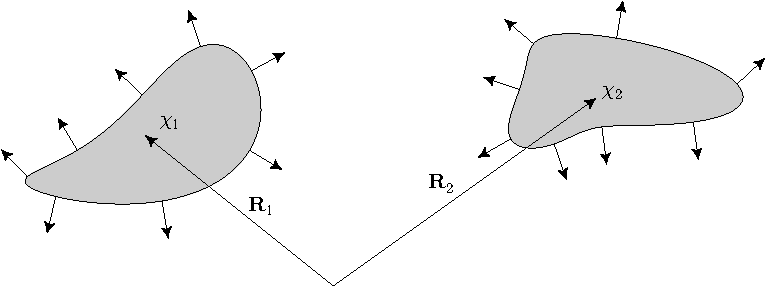
\includegraphics[width=\columnwidth]{fig/spud_sketch}
% %   \caption{Geometry for interacting dielectric bodies of susceptibility $\chi_j$, centered at
% %     $\vect{R}_j$ relative to the origin.  The surfaces mark $\sigma_j=0$, and the surface normal vectors $\hat{n}_j$
% %     are also marked.}
% %   \label{fig:spud_sketch}
% % \end{figure}

% The preceding methods offer an intuitive picture of the Casimir force,
% however they are poorly behaved as one takes the strong coupling limit.  
% For a typical path of $N$ steps pinned to the surface, approximately half 
% of the path will lie inside the body.  For $\chi\gg N$, the denominator $\langle\epsr\rangle^{-1/2}$ dominates
% the integrand, so estimate of the derivatives tends to zero as $\chi^{-1/2}$ for almost all paths.  
% Only rare paths which start on the surface, but do not enter the bulk of the body will contribute significantly.  
% As a result the estimated force goes to zero in the strong-coupling limit.
% In this section we develop an alternative expression which is better behaved in the strong-coupling
% limit and makes direct contact with prior work on Dirichlet worldlines.  


% This is exactly the construction of paths employed by Gies and Weber for computing 
% forces in the sphere-plate and cylinder-plate geometries in the Dirichlet limit~\cite{Weber2010}.  
% In that work they shift the paths so that the path just grazes the plane.  The force on the planar
% surface is computed by integrating the over the times when the path intersects the spherical or cylindrical surface.
% The expressions presented here extend their results by accounting for finite $\chi$, 
% and are framed in terms of general geometries.  

% In general, different classes of paths are important in the finite $\chi$ and strong-coupling 
% cases.  At small $\chi$, the most important path statistic is the sojourn time within the bodies,
% while in strong-coupling regime, the first-touching time is the most important statistic.    
% This is correspondence was previously used to describe the numerical convergence properties of as 
% the resolution of the paths was varied~\cite{Mackrory2016}.  
% More practically, this makes it difficult to use a single class of loops to evaluate the potential at all $\chi$:
% in weak-coupling one wants a path-ensemble that enters all of the bodies, while in strong-coupling
% it is the paths that just touch the surfaces that are most important.

% The expressions for the force in Eqs.~(\ref{eq:pinning_force}) and (\ref{eq:occupation_force})
% reflect taking two limits in different orders, namely the taking the large $N$ limit and differentiation.  
% The first derivation assumed an arbitrarily fine path where $N\gg \chi$ for all $\chi$.  Under
% differentiation the arbitrarily fine paths can be pinned to the surface, and there is a range of 
% $\cT$ where the integrand is non-zero.  However for a discrete path of length $N$, for sufficiently large $\chi$, 
% this range of $\cT$ is inaccessible, and thus the naive numerical estimate fails.    
% The second derivation instead takes the $N\rightarrow\infty$ expression last, while using well-behaved
% expressions as $\chi\rightarrow\infty$, as is better suited to a numerical method based on discrete paths.  
% This method instead highlights finding the times when the number of points inside each body 
% change.  

\subsection{Numerical Implementation of TE Casimir Forces}

\begin{align}
  \vect{F}_2 =& (-1)\frac{\hbar c N}{2(2\pi)^{D/2}}\intzinf \frac{d\cT}{\cT^{1+D/2}}
  \hspace{-2ex}\oint\limits_{\sigma_2(\vect{x}_0-\vect{R}_2)=0}  \hspace{-4ex} dS
% \nonumber\\
%   &\hspace{0.5cm}\times
  \sum_{n=0}^{N-1}\sum_{m=1}^{N-n-1}\bigdlangle\hat{n}_2(\vect{x}_0)
  \I[1]m\I[2]n f_{m,n}\bigdrangle_{\vect{x}(t)}
\end{align}
where the material dependence is carried by 
\begin{align}
  f_{m,n}&:=c_{m,n}-c_{m,n+1}-c_{0,n}+c_{0,n+1},\\
  c_{m,n} &:= \bigg( 1 + \frac{m\chi_1+n\chi_2}{N}\bigg)^{-\alpha},
\end{align}

\subsection{Numerical Implementation for TE Potential Curvature}

The path integral for the potential curvature in the occupation numbers apporach requires paths 
that are constrained by $\sigma_1(\vect{x}_j)$ and $\sigma_2(\vect{x}_k)$.  
There are a couple approaches to take here.  First, we could generate paths and then retroactively
find points close to the requisite surfaces, and perturb those paths such that the points do touch the 
surface.  We would then sum over all possible combinations of the indices close to the surfaces.
In this approach we would sample a position $x_0$, and then a time $\cT$.  Then we would find the 
near-intersections, and sum the integral over perturbing these.  

Recall, the potential curvature is 
\begin{align}
  C_{ij} =& \frac{\hbar c N}{2(2\pi)^{D/2}}\intzinf\frac{d\cT}{\cT^{1+D/2}}
  \hspace{-2ex}\oint\limits_{\sigma_2(\vect{x}_0-\vect{R}_2)=0}  \hspace{-4ex} dS\, \hat{n}_1(\vect{x}_0)
  %\nonumber\\ 
%  &\times
\biggdlangle 
  \sum_{k=0}^{N-1}\hat{n}_2(\vect{x}_k)\mathcal{G}(\vect{x}_0,\vect{x}_k,k,\cT)
  \nonumber\\
  &\hspace{0.75cm} \times\sum_{n=0}^{N-2}\sum_{m=0}^{N-n-2}\I[1]n\I[2]m g_{m,n}
  \biggdrangle_{\vect{x}(t)|\sigma_2(\vect{x}_k-\vect{R}_2)=0}
\end{align}
where 
\begin{align}
  g_{m,n}=c_{m+1,n+1}+c_{m,n}-c_{m+1,n}-c_{m,n+1},
\end{align}

That effort scales quite badly roughly as an additional $N^2$.  
We could pick the a pair of fixed indices based on their probability of occuring?  
Secondly, we could also explicitly sample from the strong-coupling limit.

This integrand is non-zero for paths that touch both bodies.  In the strong-coupling limit,
only paths that just graze the bodies will contribute.  However at finite $\chi$, all paths 
are useful since paths with a finite sojourn time contribute significantly.  

This suggests a two-fold approach: generate paths constrained to touch without regard for their
occupation time (which will capture small $\chi$), and also isolate a subset of pasth which just touch the 
bodies (which will capture large $\chi$).  

We can either directly generate the paths that obey the constraints, or we can generate 
generic paths and then check whether these paths touch the desired surfaces.  

In the second strategy, the paths are generated, and we then check if there are any points
on the path which are close to a surface.  Mathematically 
$\text{min}_x|\vect{x}_j-\sigma_b(x)|\sim \sqrt{\Delta T}$.  We would then find all such points
for both bodies and then randomly select a pair to be pinned to the surface.
 We would also have to introduce the correction
for distorting this path point to lie on the surface,
\begin{equation}  
  P_{\text{pin-corr}} = \frac{P_{\text{pinned}}}{P_{\text{free}}}
  =\frac{ e^{-|\vect{x}_{j+1}-\vect{x}^*|^2/(2\Delta T)-|\vect{x}_{j-1}-\vect{x}^*|^2/(2\Delta T)  } }
  {e^{-|\vect{x}_{j+1}-\vect{x}_j|^2/(2\Delta T)-|\vect{x}_{j-1}-\vect{x}_j|^2/(2\Delta T)  }},
\end{equation}
where $x^*$ is the nearest point to the surface to $\vect{x}_j$.

\subsubsection{Softened $\delta$-function}
There is an alternative formulation for handling the $\delta$-function.  Instead of explicitly constructing 
paths to satisfy the $\delta$-function, we can generate an effective potential.  
First consider a single integral against a Gaussian distribution, with a $\delta$-function,
\begin{align}
  I &= \int dx_j \frac{1}{2\pi\Delta\cT}
  e^{-(x_{j+1}-x_j)^2/(2\Delta \cT)-(x_{j}-x_{j+1})^2/(2\Delta \cT)} f(x_j)\delta(x_j-d) \\
&=
\frac{1}{2\pi\Delta\cT}
  e^{-(x_{j+1}-d)^2/(2\Delta \cT)-(d-x_{j+1})^2/(2\Delta \cT)} f(d).
\end{align}
While this integral can be straightforwardly evaluated, it is inconvenient within the path integral
to have to sum over explicitly pinned paths for each $x_j$.  We can circumvent this by inserting unity 
by multiplying and dividing by an integral over the Gaussian probability distribution, 
\begin{align}
  I &= \frac{1}{2\pi\Delta\cT}
  e^{-(x_{j+1}-d)^2/(2\Delta \cT)-(d-x_{j+1})^2/(2\Delta \cT)} f(d)
  \nonumber\\  &\times
\dfrac{\int dy_j (2\pi\Delta\cT)^{-1}
  e^{-(x_{j+1}-y_j)^2/(2\Delta \cT)-(y_{j}-x_{j+1})^2/(2\Delta \cT)}}{\int dy_j (2\pi\Delta\cT)^{-1}
  e^{-(x_{j+1}-y_j)^2/(2\Delta \cT)-(y_{j}-x_{j+1})^2/(2\Delta \cT)}}\\
% &= \frac{1}{2\pi\Delta\cT}
%   e^{-(x_{j+1}-d)^2/(2\Delta \cT)-(d-x_{j+1})^2/(2\Delta \cT)} f(d)
%   \left[\frac{1}{\sqrt{4\pi\Delta \cT}}e^{-(x_{j+1}-x_{j-1})^2/(4\Delta\cT)}\right]^{-1}
% \nonumber\\
% &\times\int dy_j \frac{1}{2\pi\Delta\cT}
%   e^{-(x_{j+1}-y_j)^2/(2\Delta \cT)-(y_{j}-x_{j+1})^2/(2\Delta \cT)}\\
&= \frac{1}{\sqrt{\pi\Delta\cT}}
  e^{-[d-(x_{j+1}+x_{j-1})/2]^2/\Delta \cT}f(d)
\int dy_j \frac{1}{2\pi\Delta\cT}
  e^{-(x_{j+1}-y_j)^2/(2\Delta \cT)-(y_{j}-x_{j+1})^2/(2\Delta \cT)}.
\end{align}
In the path integral one can then use free paths, where the introduced coordinate
$y_j$ replaces the constrained $x_j$ coordinate, and is subsumed within the free Gaussian path measure.
The downside is that the integrand is only non-zero
for a small range of times and positions, but this can be taken into account in the Monte Carlo sampling
strategy.  

This can be extended to handle multi-dimensional paths subject to a surface constraint, $\delta[\sigma(\vect{x})]$.
 In that case 
one multiplies and divides by the appropriate multi-dimensional Gaussian.  Since each Cartesian dimension
of the Gaussians decouples from the others, the same manipulations apply dimension-by-dimension, 
with the result
\begin{align}
  I % &= \int_{\sigma(\vect{y})=0}dS\frac{1}{|\nabla\sigma|}\frac{1}{(2\pi\Delta\cT)^D}
%   e^{-|\vect{x}_{j+1}-\vect{y}|^2/(2\Delta \cT)-|\vect{y}-\vect{x}_{j+1}|^2/(2\Delta \cT)} f(\vect{y})
%   \nonumber\\  &\times
% \dfrac{\int d\vect{x}_j \dfrac{1}{(2\pi\Delta\cT)^{D/2}}
%   e^{-|\vect{x}_{j+1}-\vect{x}_j|^2/(2\Delta \cT)-|\vect{x}_{j}-\vect{x}_{j-1}|^2/(2\Delta \cT)}}
% {\int d\vect{x}_j \dfrac{1}{(2\pi\Delta\cT)^{D/2}}
%   e^{-|\vect{x}_{j+1}-\vect{x}_j|^2/(2\Delta \cT)-|\vect{x}_{j}-\vect{x}_{j-1}|^2/(2\Delta \cT)}}\\
% &= \frac{1}{2\pi\Delta\cT}
%   e^{-(x_{j+1}-d)^2/(2\Delta \cT)-(d-x_{j+1})^2/(2\Delta \cT)} f(d)
%   \left[\frac{1}{\sqrt{4\pi\Delta \cT}}e^{-(x_{j+1}-x_{j-1})^2/(4\Delta\cT)}\right]^{-1}
% \nonumber\\
% &\times\int dy_j \frac{1}{2\pi\Delta\cT}
%   e^{-(x_{j+1}-y_j)^2/(2\Delta \cT)-(y_{j}-x_{j+1})^2/(2\Delta \cT)}\\
% &= \int_{\sigma(\vect{y})=0}dS\frac{1}{|\nabla\sigma|}\frac{1}{(\pi\Delta\cT)^{D/2}}
%   e^{-|\vect{x}_{j+1}-\vect{x}_{j-1}|^2/(4\Delta \cT)-|\vect{x}_{j+1}-\vect{y}|^2/(2\Delta \cT)-|\vect{y}-\vect{x}_{j+1}|^2/(2\Delta \cT)} f(\vect{y})\nonumber\\
%   &\times\int d\vect{x}_j \frac{1}{(2\pi\Delta\cT)^{D/2}}
%   e^{-|\vect{x}_{j+1}-\vect{x}_j|^2/(2\Delta \cT)-|\vect{x}_{j}-\vect{x}_{j-1}|^2/(2\Delta \cT)}\\
=& \int_{\sigma(\vect{y})=0}dS\frac{1}{|\nabla\sigma|}\frac{1}{(\pi\Delta\cT)^{D/2}}
  e^{-|\vect{y}-(\vect{x}_{j+1}+\vect{x}_{j-1})/2|^2/(\Delta \cT)} f(\vect{y})\nonumber\\
  &\times\int d\vect{x}_j \frac{1}{(2\pi\Delta\cT)^{D/2}}
  e^{-|\vect{x}_{j+1}-\vect{x}_j|^2/(2\Delta \cT)-|\vect{x}_{j}-\vect{x}_{j-1}|^2/(2\Delta \cT)}.
\end{align}

This allows us to use paths that are close to the surface, without exactly touching the surface.  
The integrand is still ony significant for times and paths where this occurs.  For a fixed 
starting point $\vect{x}_0$, pinning point $\vect{y}$, and path $\vect{x}_j=\vect{x_0}+\sqrt{\cT}\vect{B}_j$,
this can be converted into a probability distribution for
the allowed times, $\cT$.    
\begin{align}
  \exp\bigg[-\frac{|\vect{y}-(\vect{x}_{j+1}+\vect{x}_{j-1})/2|^2}{\Delta\cT}\bigg]
  &= \exp\bigg[-\frac{1}{\Delta\cT}|\vect{d}-\sqrt{\cT}\bar{\vect{B}}_{j}|^2\bigg] \\
  &= \exp\bigg[-N\bigg(\frac{\vect{d}^2}{\cT} -\frac{2\vect{d}\cdot\bar{\vect{B}}_j}{\sqrt{\cT}}
    + \bar{\vect{B}}_{j}^2\bigg)\bigg] \\
  &= \exp\bigg[-N|\vect{d}|^2\bigg(\frac{1}{\sqrt{\cT}} -\frac{\vect{d}\cdot\bar{\vect{B}}_j}{|\vect{d}|^2}\bigg)^2
%  \bigg]  \nonumber\\    &\times\exp\bigg[
    -N\left(\bar{\vect{B}}_{j}^2-\frac{(\vect{d}\cdot\bar{\vect{B}}_j)^2}{|\vect{d}|^2}\right)\bigg] 
\end{align}
where we introduce $\bar{\vect{B}}_j:=(\vect{B}_{j+1}+\vect{B}_{j-1})/2$ and $\vect{d}=\vect{y}-\vect{x}_0$.
The first factor is effectively Gaussian in $1/\sqrt{\cT}$, while the second factor suppresses terms where the 
path is orthogonal to line between the path starting point, and the patch on the surface.  
This second factor could in turn be used to sample from the surface for a given path.  


\subsubsection{Direct Construction of constrained paths}

Alternatively,  we can enforce the touching constraint directly and make the paths touch the bodies by constructing
paths which are fixed at steps $j$ and $k$ to touch the surface, and sum over all $j,k\in {1,N}$.  
Evidently the direct approach will create many paths with small contributions, particular if $j-k \sim 1$.
This can be made more efficient by exploiting the Gaussian factor as a probability distribution.

In computing the energy the Gaussian is introduced for the purpose of importance sampling, and must
be factored out.  In this case, the Gaussian factor is already manifest, and should be taken into account
when sampling time.s   
We would sample times from Eq.~\ref{eq:expT}, with 
\begin{equation}
  T_0 = \frac{N^2d^2}{2\Delta(N-\Delta)} \label{eq:T0_curvature}
\end{equation}
where $\Delta$ is the difference in indices at the crossing points.
The result of using this is as our probability distribution is to factour out a normalization constant,
which leaves the integrand as 
\begin{equation}
  c=\frac{N}{\sqrt{2\pi\Delta(N-\Delta)}}\Gamma(s-1)\bigg(\frac{N^2d^2}{2\Delta(N-\Delta)}\bigg)^{-s+1}
    =\frac{2^{s-1}\Gamma(s-1)}{\sqrt{2\pi} d^{2s-2}}\bigg[\frac{\Delta(N-\Delta)}{N^2}\bigg]^{s-3/2}
\end{equation}
where the exponent $s=1+(D+1)/2=7/2$ accounts for the path integral normalization and the Gaussian factors of $T$ at
zero temperature.    
The values for the difference between the pinning indices $\Delta$ are found by numerical root-finding, using bisection.
The cumulative probability distribution for $\Delta$ is
\begin{gather}
 S_\Delta = \frac{1}{S_{N-1}}\sum_{j=1}^\Delta \bigg[\frac{j(N-j)}{N^2}\bigg]^{s-3/2}
\end{gather}
Given a uniform random number $u$, the corresponding index $\Delta$ must satisfy $S_{\Delta-1}<u<S_\Delta$.
The difference $\Delta$ can be found by bisection and starting with estimates at $S_0$ and $S_{N-1}$.
The final expression for the potential curvature is
\begin{align}
  C_{ij}%   =& \frac{\hbar c}{2(2\pi)^{D/2}}\sum_{j,\Delta>0}\int \frac{d\cT}{\cT^{1+D/2}}\biggdlangle \int d\vect{x}_0
%   \frac{N^2e^{-N^2d^2/[2 \Delta(N-\Delta)\cT]}}{\sqrt{2\pi \cT \Delta(N-\Delta)}}\nonumber\\
%   &\times
%    \hat{n}_1(\vect{x}_j)\hat{n}_2(\vect{x}_{k})
%    \sum_{n=0}^{N-2}\sum_{m=0}^{N-n-2}\I[1]n\I[2]m g_{m,n}
%    \biggdrangle_{\vect{x}(\cT);{\sigma_1(\vect{x}_j-\vect{R}_1)=0\atop \sigma_2(\vect{x}_{j+\Delta}-\vect{R}_2)=0}}\\
% =& \frac{\hbar c}{2(2\pi)^{D/2}}\sum_{j}\int d\vect{x}_0\biggdlangle 
% \frac{2^{s-1}\Gamma(s-1)S_{N-1}}{\sqrt{2\pi}|\vect{x}_j-\vect{x}_{j+\Delta}|^{2(s-1)}}
%   \hat{n}_1(\vect{x}_j)\hat{n}_2(\vect{x}_{k})
%   \sum_{n=0}^{N-2}\sum_{m=0}^{N-n-2}\I[1]n\I[2]m g_{m,n}
%   \biggdrangle_{\Delta,\cT,\vect{x}(\cT);{\sigma_1(\vect{x}_j-\vect{R}_1)=0\atop \sigma_2(\vect{x}_k-\vect{R}_2)=0}},
=& \frac{\hbar c}{2(2\pi)^{D/2}}\sum_{j}\int d\vect{x}_0\biggdlangle 
\frac{3S_{N-1}}{|\vect{x}_j-\vect{x}_{j+\Delta}|^{5}}
  \hat{n}_1(\vect{x}_j)\hat{n}_2(\vect{x}_{k})
  \sum_{n=0}^{N-2}\sum_{m=0}^{N-n-2}\I[1]n\I[2]m g_{m,n}
  \biggdrangle_{\Delta,\cT,\vect{x}(\cT);{\sigma_1(\vect{x}_j-\vect{R}_1)=0\atop \sigma_2(\vect{x}_k-\vect{R}_2)=0}},
\end{align}
where we have used $\dlangle \cdots\drangle_{y; C}$ to denote ensemble averaging over quantities 
$y$ subject to possible constraints $C$.  The first pinning positions $j$ are uniformly sampled over,
the second pinnings are sampled from $P_\Delta$ with $k=j+\Delta$, and the times are sampled from
$P_{\text{exp-T}}(T;T_0,1+(D+1)/2)$, with $T_0$ given by Eq.~(\ref{eq:T0_curvature}).  
The paths are still then constructed subject to the constraints of touching the bodies at the appropriate
indices.  The remaining integrand is evaluated for the resulting paths.  

\subsubsection{Strong-Coupling Limits}

In order to capture the strong-coupling dependence it is necessary to also sample from the no-touching
set of paths.  For two half-spaces this can be constructed by shifting paths so that the minimum
point of the path starts on one body, $B(t)\rightarrow B(t) -B_{\text{min}}+d_1$.
We then find the maximum point $B_{\text{max}}$ and consider fixing that to lie on the second surface $d_2$.
Let us call the index of the maximum location $j$.

The leading exponential potential can be converted into a probability distribution for $\cT$ on a 
path-wise basis if we consider $x_j = x_0+\sqrt{\cT}B_j$, where $B_j$ is the $j$th coordinate of a 
unit Brownian bridge.   The exponential factor can be written as 
\begin{align}
  \exp\bigg\{-\frac{1}{\Delta \cT}[d-(x_{j+1}+x_{j-1})/2]^2/\Delta \cT\bigg\} 
  &= \exp\bigg\{-Nd^2\bigg[\frac{1}{\sqrt{\cT}}-\frac{\bar{B}_j}{d}\bigg]^2\bigg\},
\end{align}
where $\bar{B}_j := (B_{j+1}-B_{j-1})/2$.  This is effectively a Gaussian in $1/\sqrt{\cT}$.  
The normalized probability distribution is  
\begin{equation}
  P_C(\cT;\bar{B}_j,d,N) = \sqrt{\frac{Nd^2}{\pi\cT^3}}\exp\bigg[-Nd^2\left(\frac{1}{\sqrt{\cT}}-\frac{\bar{B}_j}{d}\right)^2\bigg],
\label{eq:time_fix_curve}
\end{equation}
for $\cT\in[0,(d/\bar{B}_j)^2]$
The probability distribution can be converted to an one-sided normal distribution by defining
\begin{equation}
  s = \sqrt{2Nd^2}\left(\frac{1}{\sqrt{\cT}}-\frac{\bar{B}_j}{d}\right),
\end{equation}
which has Jacobian (which takes the change of measure into account)
\begin{equation}
  \frac{ds}{d\cT} = \frac{-\sqrt{2Nd^2}}{2\cT^{3/2}}.
\end{equation}
In that case, $s$ is the absolute value of a standard normal deviate, and 
% \begin{equation}
%   P_C(s;B_j,d,N) = \sqrt{\frac{Nd^2}{\pi}}e^{-Nd^2s^2},
% \end{equation}
% for $s\in[0,\infty]$. 
the path-times are then given by
\begin{equation}
  \cT = \left( \frac{|z|}{\sqrt{2Nd^2}}+\frac{\bar{B}_j}{d}\right)^{-2}\label{eq:cT-s},
\end{equation}
where $z$ is a standard-normal random variable of zero mean, and unit variance.
In the strong-coupling limit, we sample from a subset of paths that just graze the surface.
With the above method of handling the $\delta$-function, there is no need for an additional Gaussian
pinning factor.  
(For planar surfaces)
\begin{align}
  C^{(S)}_{ij}  =& \frac{N\hbar c}{2(2\pi)^{D/2}}\biggdlangle \int_0^\infty \frac{d\cT}{\cT^{1+D/2}}
  \sum_j  \frac{1}{(\pi\Delta\cT)^{1/2}}
   e^{-(d-\bar{B}_j)^2/\Delta \cT}\I[1]0\I[2]0 g_{0,0}
   \biggdrangle_{x(\cT)}
 \end{align}
The $\cT$ integral will be solved in Monte Carlo fashion after factoring out the probability density~(\ref{eq:time_fix_curve}),
and using Eq.~(\ref{eq:cT-s}).  The integral can be cut off at $\cT_0:=(d/\bar{B}_j)^2$, since for $\cT>\cT_0$
more than one point has definitely entered the bodies. 
In strong-coupling, only the no-touching terms contribute, and we can use $g_{0,0}=1$.
\begin{align}
C^{(S)}_{ij} =& \frac{N\hbar c}{2(2\pi)^{D/2}}\biggdlangle  \frac{1}{\cT^{1+D/2}}
  \sum_j   \sqrt{\frac{\pi\cT^3}{Nd^2}}\sqrt{\frac{N}{\pi\cT}}
   \I[1]0\I[2]0 
   \biggdrangle_{\vect{x}(\cT), \cT}\\
 =& \frac{N\hbar c}{2(2\pi)^{D/2}}\biggdlangle  \frac{1}{\cT^{D/2}}
  \sum_j  \frac{1}{d}   \I[1]0\I[2]0 
   \biggdrangle_{\vect{x}(\cT), \cT}.
\end{align}
\comment{Phenomenologically this works relatively well if we include an additional factor of $N$.}
Note that there are no explicit restrictions on the paths, but the integral is only significant
when the paths are pass close to the body.
(For planar surface, the Gaussian integrals over $\vect{y}$ can be carried out, 
while it is necessary to factor out the cross-sectional area, and consider the second derivative 
of the energy per unit area).
\comment{scaled out areas, and integrated over }




\section{Path Construction Revisited: Path-Pinning as Importance Sampling}

In the curvature numerics, the forces emerged from paths constrained to touch the surfaces 
of the interacting bodies.  While this is a necessity for forces, constrained paths can also be used
to compute Casimir energies.
Although the Casimir energies do not require such constraints, the renormalized 
integrand is only non-zero for paths that touch both surfaces.
This suggest using paths constrained to touch both surfaces by construction.  This is a form of importance
sampling, beyond what is suggested by the Gaussian measure of the worldline path integral.
We would construct paths that are constrained to touch both surfaces, and correct for this modification
to the path integral.  In the TM Casimir energy, this is very useful, since the birth-death method 
causes many paths to be created, and ideally most of these new paths would also contribute to the path 
integral.  
In the absence of such a bias, a large number of paths are created near one surface, and if these paths
do not intersect the other body, a large amount of computational effort is wasted.  

Consider a Gaussian path integral,
\begin{equation}
  I_k=\int \frac{d\cT}{(2\pi)^{D/2}\cT^{1+D/2}}\int d\vect{x}\, f(\vect{x})P(\vect{x}),
\end{equation}
where $f$ is some function of the whole path that is only non-zero if the path enters a given region.
The $D-1$-dimensional probability density is given by,
\begin{equation}
  P(\{\vect{x}\}) = (2\pi\cT)^{(D-1)/2}\prod_{k=0}^{N-1} \frac{1}{(2\pi\Delta\cT)^{(D-1)/2}}e^{-(\vect{x}_{k+1}-\vect{x}_k)^2/(2\Delta\cT)},
\end{equation}
Instead of just taking $P$ as the probability density, let us consider using $Q=P(\vect{x})|_{x_k=d}$,
where one point is fixed on the surface of the region
\begin{align}
  Q(\{\vect{x}\}) =& (2\pi\cT)^{(D-1)/2}\cN_Q^{-1}\prod_{j=0}^{N-1}
 \frac{1}{(2\pi\Delta\cT)^{(D-1)/2}}e^{-(\vect{x}_{j+1}-\vect{x}_j)^2/(2\Delta\cT)}\bigg|_{x_k=\vect{d}},
  \end{align}
  where the normalization constant is
\begin{equation}
\cN_Q=\bigg[\frac{N^2}{2\pi k(N-k)\cT}\bigg]^{(D-1)/2}
e^{-N^2(\vect{d}-\vect{x}_0)^2/[2k(N-k)\cT]}
\end{equation}
The ratio of the probability densities is 
\begin{align}
  \frac{P}{Q} &= \cN_Q\frac{\exp\left[-\frac{(\vect{x}_{k-1}-\vect{x}_k)^2}{2\Delta \cT}
      -\frac{(\vect{x}_{k}-\vect{x}_{k+1})^2}{2\Delta \cT}\right]}
  {\exp\left[-\frac{(\vect{x}_{k-1}-\vect{d})^2}{2\Delta \cT}
      -\frac{(\vect{d}-\vect{x}_{k+1})^2}{2\Delta \cT}\right]}
%  \\  &
= \cN_Q\exp\left[-\frac{(\vect{x}_{k}-\bar{\vect{x}})^2}{\Delta \cT}
      +\frac{(\vect{d}-\bar{\vect{x}})^2}{\Delta \cT}\right].
\end{align}
% Note that the paths are constructed to ensure $\vect{x}_0\rightarrow\vect{d}$.  There is still one 
% remaining integral which can also be sampled from in determining the integrand, but this sampled $\vect{x}_k$
% does not alter the path.  

The resulting integrand could be built up from Monte Carlo samples 
\begin{equation}
  I_k = \int \frac{d\cT}{(2\pi)^{D/2}\cT^{1+D/2}}\int d\vect{x}_k\, \cN_Q e^{-\frac{(\vect{x}_{k}-\bar{\vect{x}})^2}{\Delta \cT}
      +\frac{(\vect{d}-\bar{\vect{x}})^2}{\Delta \cT}} f(\vect{x})Q(\vect{x})
\end{equation}
The normalization $\cN_Q$ can be used to sample the times, with $s=D/2$ and $\cT_0=N^2|\vect{d-x}_0|^2/[2k(N-k)]$ as the distribution
parameters.
The remaining $\vect{x}_k$ integral can be evaluated by using the Gaussian.
However, those sampled values of $\vect{x}_k$ are not the path values, rather they are sampled after
the path is constructed subject to the pinning requirement.    
The appropriate integrand for Monte carlo in pinned paths, $\vect{x}_k$ and times $\cT$ is 
\begin{align}
  I_k &= \dlangle \frac{\Gamma[D/2]}{\cT_0^{D/2}}\bigg(\frac{N}{2\pi k (N-k)\Delta\cT}\bigg)^{(D-1)/2}
  (\pi \Delta\cT)^{(D-1)/2} e^{\frac{(\vect{d}-\bar{\vect{x}})^2}{\Delta \cT}} f(\vect{x})\drangle_{\{\vect{x}\}',\vect{x}_k,\cT}\nonumber\\
   % &= \dlangle \Gamma[D/2] \left(\frac{2k(N-k)}{N^2\vect{|d-x_0|}^2}\right)^{D/2} \frac{N^{n/2}}{[2k(N-k)]^{n/2}}
   %  e^{\frac{(\vect{d}-\bar{\vect{x}})^2}{\Delta \cT}} f(\vect{x})\drangle_{\{\vect{x}\}',\vect{x}_k}\\
   &= \dlangle \Gamma[D/2] \frac{[2k(N-k)]^{(D-n)/2}}{N^{D-n/2}\vect{|d-x_0|}^D}   
   e^{\frac{(\vect{d}-\bar{\vect{x}})^2}{\Delta \cT}} f(\vect{x})\drangle_{\{\vect{x}\}',\vect{x}_k,\cT}.
 \end{align}

Of course, if the pinned point is also integrated over (such as the transverse dimensions for a planar medium),
 then a different distance dependence.
  In that case, only one dimension remains to be evaluated in the path integral,
% \begin{align}
%   I   &= \dlangle \Gamma[D/2] \frac{[2k(N-k)]^{(D-1)/2}}{N^{D-1/2}|d-x_0|^D}   
%   e^{\frac{(\vect{d}-\bar{\vect{x}})^2}{\Delta \cT}} f(\vect{x})\drangle_{\{\vect{x}\}',\vect{x}_k,\cT}.
% \end{align}
The result can be written out explicitly for $D=4$
\begin{align}
  I   &= \dlangle  \frac{[2k(N-k)]^{3/2}}{N^{2}N^{3/2}|d-x_0|^4}   
  e^{\frac{(\vect{d}-\bar{\vect{x}})^2}{\Delta \cT}} f(\vect{x})\drangle_{\{\vect{x}\}',\vect{x}_k,\cT}.
\end{align}

The above development fixed one particular index $k$.  This index $k$ can also be sampled over to vary
which points are pinned to the surface.  We propose using $P_k= 6 k(N-k)/N^2$, as this is simple to sample
from and is not too sharpled peaked around $k=N/2$.
\comment{need to integrate over surface, changes normalization, changes dimension of normalization $\implies$
  leftover $k$ dependence}

% The normalization for path subject to a single constraint is 
% \begin{equation}
%   \mathcal{N}_1=\mathcal{G}\big[\vect{x}_0,\vect{d},k(N-k)\cT/N^2\big],
% \end{equation}
% exactly as emerged for the potential curvature.  We will use this to sample times
% as described in Sec.~\ref{sec:expT-sampling}.

% The normalization for the $Q$ probability distribution is 
% \begin{equation}
%   \cN =\frac{1}{[2\pi k \Delta \cT]^{D/2}[2\pi (N-k)\Delta \cT]^{D/2}}
%     e^{-N^2(\vect{x}_0-\vect{d})^2/(2k(N-k) \cT)}
% \end{equation}
% (a factor of $[2\pi\cT]^{D/2}$ mutliplies this if that is factored out for the usual Brownian bridge
% normalization).  This is the probability we must factor out to sample bridges for where the $k^{\text{th}}$ point
% is fixed.  
% Use that as basis to sample times, and indices.

\section{Numerical Methods: Accelerated Convergence}

This analytical could be applied to enhance Dirichlet worldline methods with little cost,
since path resolution is one of the dominant sources of error in numerical worldlines~\cite{Mackrory2016}.






%%% Local Variables: 
%%% mode: latex
%%% TeX-master: "thesis_master"
%%% End: 
